%%%%%%%%%%%%%%%%%%%%%%%%%%%%%%%%%%%%%%%%%%%%%%%%%%
%% Bachelor's & Master's Thesis Template        %%
%% Copyleft by Dawid Weiss & Marta Szachniuk    %%
%% Faculty of Computing and Telecommunication   %%
%% Poznan University of Technology, 2020        %%
%%%%%%%%%%%%%%%%%%%%%%%%%%%%%%%%%%%%%%%%%%%%%%%%%%


% Szkielet dla pracy licencjackiej pisanej w języku polskim.

\documentclass[polish,bachelor,a4paper,oneside]{ppfcmthesis}


\usepackage[utf8]{inputenc}
\usepackage[OT4]{fontenc}
\usepackage{hyperref}

\hypersetup{
    colorlinks=false, %set true if you want colored links
    linktoc=all,     %set to all if you want both sections and subsections linked
    linkcolor=black,  %choose some color if you want links to stand out
}

%--------------------------------------
% Strona tytułowa
%--------------------------------------

% Autorzy pracy, jeśli jest ich więcej niż jeden
% wstaw między nimi separator \and
\author{%
   Mateusz Biernacki \album{140681} \and 
   Dominik Boła \album{136524} \and 
   Maciej Goral \album{132228} \and 
   Grzegorz Piątkowski \album{135868}}
\authortitle{}                                % Do not change.

\title{Aplikacja internetowa służąca do generowania planów lekcji dla szkół podstawowych oraz średnich}

% Your supervisor comes here.
\ppsupervisor{~dr~inż.~Izabela Janicka-Lipska} 

% Year of final submission (not graduation!)
\ppyear{2022}                                 


\begin{document}

% Front matter starts here
\frontmatter\pagestyle{empty}%
\maketitle\cleardoublepage%

%--------------------------------------
% Miejsce na kartę pracy dyplomowej
%--------------------------------------

\thispagestyle{empty}\vspace*{\fill}%
\begin{center}Tutaj będzie karta pracy dyplomowej;\\oryginał wstawiamy do wersji dla archiwum PP, w pozostałych kopiach wstawiamy ksero.\end{center}%
\vfill\cleardoublepage%

%--------------------------------------
% Spis treści
%--------------------------------------

\pagenumbering{Roman}\pagestyle{ppfcmthesis}%
\tableofcontents* 
\cleardoublepage % Zaczynamy od nieparzystej strony

%--------------------------------------
% Rozdziały
%--------------------------------------

%Najwygodniej jeśli każdy rozdział znajduje się w oddzielnym pliku
\mainmatter%

\chapter{Wstęp}
(Źródła?)Tematem podjętym w pracy jest aplikacja służąca do generowania planów zajęć. Główną motywacją do podjęcia takiego (tego?,"") tematu stanowią wady obecnie stosowanego przez większość szkół manualnego tworzenia planów zajęć. Ręczne tworzenie planu jest czasochłonne i wymaga dużego nakładu pracy. Dla osób odpowiedzialnych za ich przygotowanie (dalej zwanymi planistami) jest to zadanie monotonne, a także przytłaczające. Planiści, nawet ci z dużym doświadczeniem, nie są zdolni do utworzenia planu, który optymalnie wykorzystywałby godziny uczniów, nauczycieli, a także dostępność sali lekcyjnych. Skutkuje to znaczną liczbą niewykorzystanego czasu w środku dnia lekcyjnego.

Celem pracy jest zaprojektowanie aplikacji, dzięki której po podaniu niezbędnych danych, możliwe byłoby automatyczne wygenerowanie planu zajęć dla szkoły. Aplikacja ma umożliwić planiście dodawanie danych o przedmiotach, nauczycielach, salach i klasach. Na podstawie podanych danych planista ma mieć możliwość generacji rozkładu zajęć dla wszystkich klas w szkole. Aplikacja ma być przeznaczona dla szkół podstawowych oraz średnich. Ograniczenie to wynika z założenia niepodzielności klasy. W przypadku uczelni wyższych niejednolity podział na grupy znacząco zwiększa poziom skomplikowania rozwiązywanego problemu.

Praca ma następującą strukturę. Rozdział drugi poświecony jest podstawom teoretycznym. Rozdział trzeci zawiera analizę problemu i dostępnych rozwiązań. Rozdział czwarty to opis metodologii pracy. Rozdział piąty omawia część fronendową aplikacji. Rozdział szósty charakteryzuje backend aplikacji. Rozdział siódmy wyjaśnia działanie algorytmu generacji planu. Rozdział ośmy stanowią wnioski. Rozdział dziewiąty jest podumowaniem pracy. 

Implementacja aplikacji została wykonana przez cztery osoby.
Mateusz Biernacki wykonał ...
Dominik Boła wykonał ...
Maciej Goral wykonał ...
Grzegorz Piątkowski wykonał ...

Wstęp do pracy powinien zawierać następujące elementy:
\begin{itemize}
    \item krótkie uzasadnienie podjęcia tematu; 
    \item cel pracy (patrz niżej); 
    \item zakres (przedmiotowy, podmiotowy, czasowy) wyjaśniający, w jakim rozmiarze praca będzie realizowana; 
    \item ewentualne hipotezy, które autor zamierza sprawdzić lub udowodnić; 
    \item krótką charakterystykę źródeł, zwłaszcza literaturowych; 
    \item układ pracy (patrz niżej), czyli zwięzłą charakterystykę zawartości poszczególnych rozdziałów; 
    \item ewentualne uwagi dotyczące realizacji tematu pracy np.~trudności, które pojawiły się w trakcie 
    realizacji poszczególnych zadań, uwagi dotyczące wykorzystywanego sprzętu, współpraca z firmami zewnętrznymi. 
\end{itemize}

\noindent
\textbf{Wstęp do pracy musi się kończyć dwoma następującymi akapitami:}
\begin{quote}
Celem pracy jest opracowanie / wykonanie analizy / zaprojektowanie / ...........
\end{quote}
oraz:
\begin{quote}
Struktura pracy jest następująca. W rozdziale 2 przedstawiono przegląd literatury na temat ........ 
Rozdział 3 jest poświęcony ....... (kilka zdań). 
Rozdział 4 zawiera ..... (kilka zdań) ............ itd. 
Rozdział X stanowi podsumowanie pracy. 
\end{quote}

W przypadku prac inżynierskich zespołowych lub magisterskich 2-osobowych, po tych dwóch w/w akapitach 
musi w pracy znaleźć się akapit, w którym będzie opisany udział w pracy poszczególnych członków zespołu. Na przykład:

\begin{quote}
Jan Kowalski w ramach niniejszej pracy wykonał projekt tego i tego, opracował ......
Grzegorz Brzęczyszczykiewicz wykonał ......, itd. 
\end{quote}


% Co to jest NP - https://dbpedia.org/page/NP_(complexity)
% Co to jest problem NP-Trudny - https://www.baeldung.com/cs/p-np-np-complete-np-hard
% Ułozenie planu zajęć jako problem np-trudny - https://www.sciencedirect.com/science/article/pii/S1110016816000703#b0015


\chapter{Podstawy teoretyczne}
\section{Problem optymalizacyjny}
Problem optymalizacyjny~\cite{optimization_problem} jest to problem obliczeniowy, który polega na znalezieniu maksymalnej/minimalnej wartości pewnego parametru. Wartość takiego parametru zazwyczaj opisywana jest funkcją, dzięki której wartość parametru zależna jest od przeszukiwanych danych wejściowych. Jeśli poszukiwana jest jak najmniejsza wartość parametru, mówimy o problemie minimalizacyjnym i odpowiednio w przypadku poszukiwania największej wartości parametru, mówimy o problemie maksymalizacyjnym.

\section{Problem NP-trudny}
Problem NP-trudny~\cite{np_hard} jest problemem obliczeniowym, dla którego nie jest możliwym znalezienie rozwiązania w czasie wielomianowym przy wykorzystaniu niedeterministycznej maszyny Turinga, a sprawdzenie znalezionego rozwiązania jest co najmniej tak trudne jak każdego innego problemu z grupy NP. Problem optymalizacyjny jest jednym z problemów należących do grupy NP-trudnych.

\section{Heurystyka}
Heurystyka~\cite{heuristic} jest techniką rozwiązywania problemów w przypadku, gdy znalezienie dokładnego rozwiązania jest zbyt kosztowne. Metoda heurystyczna oferuje zmniejszenie kosztów rozwiązania problemu, jednak ceną takiego podejścia jest spadek dokładności rozwiązania czy nawet jego poprawności.  Przy wykorzystaniu metody heurystycznej otrzymanie optymalnego rozwiązania możliwe jest tylko w szczególnych przypadkach. Tego typu podejście wykorzystuje się również, w przypadku, gdy algorytm dokładny umożliwiający znalezienie rozwiązania optymalnego nie jest znany, w celu zawężenia pola badań.

\section{Algorytm ewolucyjny}
Algorytm ewolucyjny~\cite{evolution_algorithm} jest heurystycznym podejściem do rozwiązywania problemów, które nie mogą zostać rozwiązane w czasie wielomianowym, takie jak grupa problemów NP-trudnych, czy po prostu w celu zmniejszenia kosztów znalezienia rozwiązania problemu. Algorytmy ewolucyjne stosowane samodzielnie używane są zazwyczaj do rozwiązywania problemów optymalizacyjnych. Zastosowanie i działanie algorytmu ewolucyjnego jest bardzo proste do zrozumienia ze względu na to, że mamy do czynienia na co dzień z podobnym zjawiskiem w naturze czyli z selekcją naturalną. Przebieg działania algorytmu ewolucyjnego składa się z 4 głównych kroków.
	\begin{enumerate}
	\item \textbf{Inizjalizacja} -- W celu rozpoczęcia działania algorytmu, potrzebna jest pierwsza grupa rozwiązań (dalej nazywana populacją). Populacja zwierać będzie założoną liczbę możliwych rozwiązań (dalej nazywaną osobnikami). Zazwyczaj podczas inicjalizacji osobniki tworzone są w sposób losowy. Takie podejście jest wręcz zalecane, ponieważ umożliwia to przebadanie dużej różnorodności osobników, dzięki czemu finałowe rozwiązanie będzie lepsze.
	\item \textbf{Selekcja} -- Gdy pierwotna populacja jest gotowa, jej osobniki trzeba poddać ocenie. Funkcja oceny powinna składać się ze ściśle opisanych warunków opisujących środowisko, do którego osobniki muszą się przystosować. Im dokładniej środowisko zostanie opisane w funkcji oceny, tym lepsze będzie finalne rozwiązanie. Gdy funkcja jest poprawnie przygotowana, każdy z osobników musi zostać poddany ocenie, po której otrzymuje parametr oceny. Dzięki temu można wyróżnić rozwiązania lepsze od reszty. Z populacji zostaje wybrana założona liczba osobników o najwyższym parametrze oceny. Reszta osobników zostaje zabita.
	\item \textbf{Ewolucja} -- Ewolucja składa się z dwóch kroków: krzyżowania oraz mutacji. 
	\begin{enumerate}
		\item Krzyżowanie -- po otrzymaniu wybranych osobników z selekcji, użyte są one do stworzenia nowego pokolenia dla algorytmu, stając się osobnikami-rodzicami. Wykorzystując charakterystyki osobników-rodziców, utworzona zostaje populacja osobników-dzieci poprzez wymieszanie ze sobą charakterystyk osobników-rodziców. Po utworzeniu nowego pokolenia osobników-dzieci, osobniki-rodzice zostają zabite.
		\item Mutacja -- jest to prawdopodobnie najważniejszy krok ewolucji. Bez niego cała populacja bardzo szybko utknęłaby w miejscu, nie oferując żadnego sensownego rozwiązania. W tym kroku charakterystyka każdego osobnika-dziecka z nowego pokolenia poddana jest małym losowym zmianom w celu zróżnicowania ich od osobników-rodziców. Na końcu tego kroku osobniki-dzieci stają się nowym pokoleniem osobników w populacji, która może ponownie zostać poddana selekcji.
	\end{enumerate}
	\item \textbf{Finalizacja} -- Ostatecznie działanie algorytmu musi dobiec końca. W tym kroku z populacji zostaje wybrany osobnik z najwyższym parametrem oceny i zwrócony jako rozwiązanie. Są dwie możliwości, w których zakończenie działania algorytmu może zostać wywołane. Gdy osiągnie on maksymalny czas działania (np. założona maksymalna liczba pokoleń) lub gdy osiągnięty zostanie poszukiwany pułap parametru oceny.
	\end{enumerate}	



\chapter{Analiza i porównanie możliwych rozwiązań}
\section{Analiza problemu}
Podstawowym problemem w automatycznym tworzeniu planu zajęć jest dobór warunków wykorzystywanych przy generacji. Warunki te można podzielić na niezbędne do utworzenia poprawnego planu oraz warunki dodatkowe, których spełnienie zwiększa użyteczność planu z punktu widzenia planisty. 

Wśród warunków niezbędnych należy wyróżnić warunek braku konfliktów. Konflikt ma miejsce, gdy występuje jedna z następujących sytuacji:
\begin{itemize}
    \item w jednej godzinie lekcyjnej, jednej klasie został przyporządkowany więcej niż jeden przedmiot,
    \item w jednej godzinie lekcyjnej, jednemu nauczycielowi została przyporządkowana więcej niż jedna klasa,
    \item w jednej godzinie lekcyjnej, jednej sali została przyporządkowana więcej niż jedna klasa.
\end{itemize}
W przypadku szkół podstawowych oraz średnich do warunków niezbędnych należy również zaliczyć brak niewykorzystanych godzin w środku dnia lekcyjnego uczniów. Dodatkowo niektóre zajęcia, takie jak wychowanie fizyczne, mogą być przeprowadzone tylko w specjalnie przeznaczonych do tego salach.

Warunki dodatkowe mogą różnić się w zależności od czynników, które należy wziąć pod uwagę przy pod uwagę przy generacji plany wynikających ze specyfikacji szkoły oraz wymagań personelu dydaktycznego. Do tych czynników można zaliczyć:
\begin{itemize}
    \item ograniczenia dostępności nauczycieli, wynikające z pracy w innych placówkach oświatowych lub innych powodów,
    \item ograniczenia wynikające z odległości między salami,
    \item obecność zajęć nieobowiązkowych, które muszą w danym dniu lekcyjnym być skrajnie pierwsze lub ostatnie,
    \item  konieczność minimalizacji niewykorzystanych godzin w środku dnia lekcyjnego dla uczniów,
    \item konieczność grupowania zajęć w przypadku kilku godzin lekcyjnych tego samego przedmiotu jednego dnia -- w takim przypadku zajęcia te powinny następować bezpośrednio po sobie oraz w tej samej sali,
    \item konieczność równomiernego rozłożenie przedmiotów w trakcie tygodnia lekcyjnego.
\end{itemize}
\section{Aktualnie dostępne rozwiązania}
\subsection{aSc TimeTables}
aSc TimeTables~\cite{asc} to aplikacja desktopowa wspomagająca przygotowywanie planów zajęć. Narzędzie umożliwia generowanie planów na podstawie zdefiniowanych wymagań, wprowadzenie do nich ręcznych poprawek oraz wyszukiwanie konfliktów we wprowadzonych zmianach. aSc TimeTables jest najbardziej rozbudowanym rozwiązaniem tego typu dostępnym na rynku, pozwalającym na tworzenie planów zajęć dla szkół i uczelni. Do dodatkowych funkcji programu należy możliwość importu danych z pliku, zdolność mapowania szkoły oraz udostępnienia planów uczniom i nauczycielom za pomocą aplikacji mobilnej. Z wszechstronnością i bogactwem funkcji wiąże się wysoki poziom umiejętności potrzebny do poprawnego wykorzystania aplikacji. Do pozostałych wad programu należy brak regularnych aktualizacji, podatność na błędy w generacji planu, wysoka cena oraz dostępność ograniczona do systemu Windows.
\subsection{Prime Timetable}
Prime Timetables~\cite{prime} to aplikacja internetowa przeznaczona dla organizacji edukacyjnych umożliwiająca zarówno ręczne jak i automatyczne układanie planów lekcji. Prime Timetables pozwala na wspólne tworzenie planów przez kilku użytkowników oraz udostępnianie gotowych planów dla uczniów i nauczycieli posiadających konta w serwisie. Aplikacja posiada rozbudowany zestaw narzędzi umożliwiających określanie ograniczeń związanych z automatyczną generacją planu. Główną wadą rozwiązania jest wysoka opłata miesięczna, której wysokość dodatkowo zależy od liczby nauczycieli w szkole. 
\subsection{SuperSaas}
SuperSaas~\cite{saas} to program do zarządzania szkołami i innymi instytucjami, którego głównym atutem jest wbudowany system rezerwacji. Przy pomocy konta WordPress użytkownicy aplikacji mogą umawiać terminy wizyt, a także dokonywać za nie płatności. SuperSaas cechuje niska cena oraz dostępność z poziomu przeglądarki. Duża część funkcjonalności aplikacji nie jest przeznaczona dla szkół. Pomimo możliwości wspomagania ręcznego układania planów zajęć, program nie pozwala na automatyczną ich generację, ani nawet wykrywanie konfliktów. 
\section{Możliwe podejścia}
Możliwe rozwiązania można podzielić w zależności od kilku aspektów. Pierwszym z nich jest wybór rodzaju aplikacji -- desktopowej, mobilnej lub internetowej. Ze względu na fakt, że korzystanie z aplikacji wymagać ma wprowadzania dużej ilości danych, można założyć, że z punktu widzenia użytkownika najkorzystniejsze będzie użycie w tym celu fizycznej klawiatury. Powoduje to odrzucenie wyboru aplikacji mobilnej. Zaletami  wyboru aplikacji desktopowej jest możliwość korzystania z niej bez dostępu do Internetu oraz bezpieczeństwo związane z lokalnym przechowywaniem danych. Pomimo tych korzyści rozwiązanie to nie oferuje zalet związanych z wyborem aplikacji internetowej -- dostępu z dowolnego urządzenia wyposażonego w kompatybilną przeglądarkę, braku wymagań systemowych związanych z obliczeniami i przechowywaniem danych oraz braku konieczności aktualizowania aplikacji przez użytkownika. Te czynniki jednoznacznie przesądzają o wykorzystaniu w projekcie aplikacji internetowej.

Drugim aspektem, który należy rozpatrzyć jest poziom złożoności aplikacji, związany głównie z wyborem możliwych do wprowadzenia przez planistę warunków wykorzystywanych przy generacji planu. Większa liczba warunków może wiązać się z lepszą jakością planu, ale także dłuższym czasem jego generacji. Należy również rozpatrzyć stosunek nakładu pracy przeznaczonej na implementację warunku w stosunku do potencjalnego zysku dla użytkowników. Każdy dodatkowy warunek spowodowałby zmniejszenie przejrzystości interfejsu graficznego, szczególnie dla użytkowników, dla których byłby on zbędny. Biorąc pod uwagę te czynniki w projekcie wykorzystane zostaną jedynie te warunki, których obecność jest niezbędna do poprawnej generacji planu.

Ostatnim ważnym do rozpatrzenia aspektem jest wybór użytkowników, którzy będą posiadać konta w systemie. Pierwszym z nich jest planista -- osoba odpowiedzialna za układanie planów. W rozwiązaniu, w których planiści nie posiadają kont, wprowadzone informacje nie byłyby przechowywane w bazie w danych, co oznacza ich utratę przypadku zakończenia sesji. Konieczność posiadania przez planistę konta eliminuje ten problem i dodatkowo utrudnia ataki na stronę. Pozostali potencjalni użytkownicy to nauczyciele oraz uczniowie. W projekcie zakładamy możliwość podania przez nauczyciela swojej dyspozycyjności. Ze względu na konieczność podania przez planistów adresu e-mail każdego dodanego nauczyciela, jest to możliwe poprzez unikatowy link wysłany w wiadomości, bez obowiązku zakładania konta. Dla uczniów, ze względu na brak bezpośredniego wpływu na plan zajęć, również nie zakłada się możliwości stworzenia konta. 
\section{Wymagania funkcjonalne i niefunkcjonalne}
Wymagania funkcjonalne:
\begin{itemize}
    \item możliwość rejestracji w aplikacji,
    \item możliwość logowania w aplikacji,
    \item możliwość dodania danych przedmiotów, nauczycieli, sal i klas,
    \item możliwość edycji danych przedmiotów, nauczycieli, sal i klas,
    \item możliwość usunięcia danych przedmiotów, nauczycieli, sal i klas,
    \item możliwość generacji planu na podstawie podanych danych,
     \item możliwość wyświetlania wygenerowanych planów z podziałem na plany dla klas, nauczycieli i sale,
    \item możliwość przesłania do nauczycieli ankiet dyspozycyjności,
    \item możliwość wypełnienia ankiety dyspozycyjności przez nauczyciela.
\end{itemize}
Wymagania niefunkcjonalne:
\begin{itemize}
    \item responsywność na urządzeniach mobilnych,
    \item uwierzytelnianie oparte o tokeny JWT,
    \item możliwość przerwania dodawania danych bez utraty postępu,
    \item kompatybilność z przeglądarkami Chrome, Firefox, Opera oraz Edge,
    \item formularze dodawania danych proste i intuicyjne w obsłudze,
    \item szyfrowanie danych w bazie danych.
\end{itemize}
\section{Przypadki użycia}
Na rysunku~\ref{rys:vuex} przedstawiono diagram przypadków użycia.
\begin{figure}[!ht]
\centering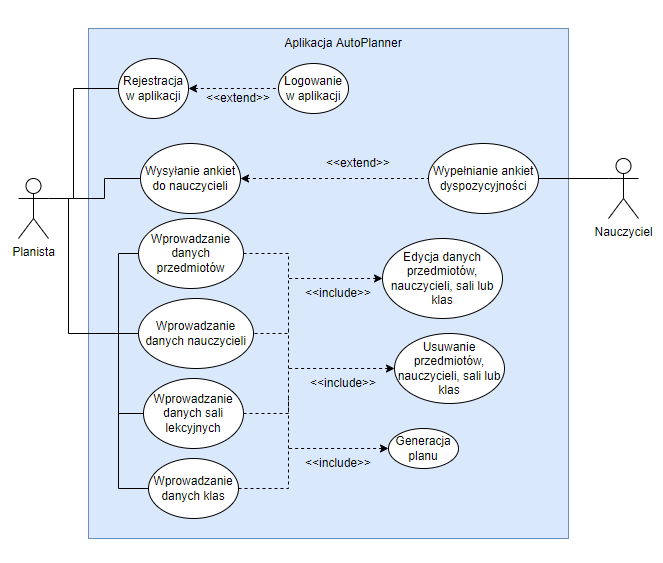
\includegraphics[width=\textwidth]{figures/DiagramPU}
\caption{Diagram przypadków użycia}\label{rys:pu}
\end{figure}


\noindent
\textbf{Przypadek użycia:} Rejestracja w aplikacji\\
\textbf{Aktor główny:} Planista\\
\textbf{Scenariusz główny:}
\begin{enumerate}
	\item Planista wpisuje adres e-mail.
	\item Aplikacja nie zgłasza problemu ze składnią adresu e-mail.
	\item Planista wpisuje nazwę użytkownika oraz hasło.
	\item Planista zatwierdza wprowadzone dane.
	\item Aplikacja akceptuje wprowadzone dane.
	\item Aplikacja tworzy nowe konto użytkownika.
\end{enumerate}
\textbf{Rozszerzenia:}
	\begin{enumerate}
         \item[2.A] Aplikacja zgłasza problem ze składnią adresu e-mail.
         \begin{enumerate}
         	\item[2.A.1] Planista poprawia składnię adresu e-mail.
         \end{enumerate}
         \item[5.A] Aplikacja zgłasza problem  dotyczący wymagań hasła.
         \begin{enumerate}
         	\item[5.A.1] Planista wpisuje hasło, które spełnia wymagania.
         \end{enumerate}
         \item[5.B] Aplikacja zgłasza, że na wpisany adres e-mail jest już założone konto.
         \begin{enumerate}
         	\item[5.B.1] Planista wpisuje nowy adres e-mail.
         \end{enumerate}
	\end{enumerate}
	
\noindent
\textbf{Przypadek użycia:} Logowanie w aplikacji\\
\textbf{Aktor główny:} Planista\\
\textbf{Scenariusz główny:}
\begin{enumerate}
	\item Planista wpisuje adres e-mail.
	\item Planista wpisuje hasło.
	\item Planista zatwierdza wprowadzone dane.
	\item Aplikacja akceptuje wprowadzone dane.
	\item Aplikacja przechodzi do widoku użytkownika zalogowanego.
\end{enumerate}
\textbf{Rozszerzenia:}
	\begin{enumerate}
         \item[4.A] Aplikacja zgłasza, że wprowadzone hasło jest nieprawidłowe.
         \begin{enumerate}
         	\item[4.A.1] Planista ponownie wpisuje hasło.
         \end{enumerate}
         \item[4.B] Aplikacja zgłasza, że użytkownik o podanym adresie e-mail nie istnieje.
         \begin{enumerate}
         	\item[4.B.1] Planista ponownie wpisuje adres e-mail.
         \end{enumerate}
	\end{enumerate}
	
\noindent
\textbf{Przypadek użycia:} Wprowadzanie danych przedmiotów\\
\textbf{Aktor główny:} Planista\\
\textbf{Scenariusz główny:}
\begin{enumerate}
	\item Planista wpisuje nazwę przedmiotu.
	\item Planista zatwierdza wprowadzone dane.
	\item Aplikacja akceptuje wprowadzone dane.
	\item Aplikacja dodaje przedmiot do listy z lewej strony ekranu.
\end{enumerate}
\textbf{Rozszerzenia:}
	\begin{enumerate}
         \item[3.A] Aplikacja zgłasza, że przedmiot o danej nazwie został już wcześniej wprowadzony.
         \begin{enumerate}
         	\item[3.A.1] Planista wpisuje nową nazwę przedmiotu.
         \end{enumerate}
         \item[3.B] Aplikacja zgłasza, że nazwa przedmiotu zawiera niedozwolone znaki.
         \begin{enumerate}
         	\item[3.B.1] Planista wpisuje nową nazwę przedmiotu.
         \end{enumerate}
	\end{enumerate}
	
\noindent
\textbf{Przypadek użycia:} Wprowadzanie danych nauczycieli\\
\textbf{Aktor główny:} Planista\\
\textbf{Scenariusz główny:}
\begin{enumerate}
	\item Planista wpisuje imię i nazwisko nauczyciela.
	\item Planista wpisuje adres e-mail nauczyciela.
	\item Aplikacja nie zgłasza problemu ze składnią adresu e-mail.
	\item Planista wybiera z listy wprowadzony przez nauczyciela przedmiot.
	\item Aplikacja akceptuje wprowadzone dane.
	\item Aplikacja dodaje nauczyciela do listy z lewej strony ekranu.
\end{enumerate}
\textbf{Rozszerzenia:}
	\begin{enumerate}
         \item[3.A] Aplikacja zgłasza problem ze składnią adresu e-mail.
         \begin{enumerate}
         	\item[3.A.1] Planista poprawia składnię adresu e-mail.
         \end{enumerate}
         \item[4.A] Planista dodaje kolejne przedmioty prowadzone przez nauczyciela.
         \item[5.A] Aplikacja zgłasza, że nauczyciel o danym adresie e-mail został już wcześniej wprowadzony.
         \begin{enumerate}
         	\item[5.A.1] Planista wpisuje nowy adres e-mail.
         \end{enumerate}
         \item[5.B] Aplikacja zgłasza, że imię lub nazwisko nauczyciela zawiera niedozwolone znaki.
         \begin{enumerate}
         	\item[5.B.1] Planista wpisuje nowe imię i nazwisko nauczyciela.
         \end{enumerate}
	\end{enumerate}

\noindent
\textbf{Przypadek użycia:} Wprowadzanie danych sal lekcyjnych\\
\textbf{Aktor główny:} Planista\\
\textbf{Scenariusz główny:}
\begin{enumerate}
	\item Planista wpisuje nazwę sali.
	\item Planista nie dodaje preferowanych przedmiotów.
	\item Planista zatwierdza wprowadzone dane.
	\item Aplikacja akceptuje wprowadzone dane.
	\item Aplikacja dodaje salę do listy z lewej strony ekranu.
\end{enumerate}
\textbf{Rozszerzenia:}
	\begin{enumerate}
         \item[2.A] Planista dodaje jeden lub więcej preferowany przedmiot.
         \item[4.A] Aplikacja zgłasza, że sala o danej nazwie została już wcześniej wprowadzona.
         \begin{enumerate}
         	\item[4.A.1] Planista wpisuje nową nazwę sali.
         \end{enumerate}
         \item[4.B] Aplikacja zgłasza, że nazwa sali zawiera niedozwolone znaki.
         \begin{enumerate}
         	\item[4.B.1] Planista wpisuje nową nazwę sali.
         \end{enumerate}
	\end{enumerate}
	
\noindent
\textbf{Przypadek użycia:} Wprowadzanie danych klas\\
\textbf{Aktor główny:} Planista\\
\textbf{Scenariusz główny:}
\begin{enumerate}
	\item Planista wpisuje nazwę klasy.
	\item Planista wybiera z listy kolejne przedmioty.
	\item Planista wpisuje tygodniowe liczby godzin dla każdego przedmiotu.
	\item Planista nie wybiera prowadzącego dany przedmiot.
	\item Planista zatwierdza wprowadzone dane.
	\item Aplikacja akceptuje wprowadzone dane.
	\item Aplikacja dodaje klasę do listy z lewej strony ekranu.
\end{enumerate}
\textbf{Rozszerzenia:}
	\begin{enumerate}
         \item[4.A] Planista wybiera z listy prowadzącego przedmiot.
         \item[6.A] Aplikacja zgłasza, że klasa o danej nazwie została już wcześniej wprowadzona.
         \begin{enumerate}
         	\item[6.A.1] Planista wpisuje nową nazwę klasy.
         \end{enumerate}
         \item[6.B] Aplikacja zgłasza, że nazwa klasy zawiera niedozwolone znaki.
         \begin{enumerate}
         	\item[6.B.1] Planista wpisuje nową nazwę klasy.
         \end{enumerate}
         \item[6.C] Aplikacja zgłasza, że wprowadzona liczba godzin ma nieprawidłowy format.
         \begin{enumerate}
         	\item[6.C.1] Planista wpisuje nową liczbę godzin.
         \end{enumerate}
	\end{enumerate}
	
\noindent
\textbf{Przypadek użycia:} Edycja danych przedmiotów, nauczycieli, sal lub klas\\
\textbf{Aktor główny:} Planista\\
\textbf{Scenariusz główny:}
\begin{enumerate}
	\item Planista wybiera przedmiot, nauczyciela, salę lub klasę, których dane chce edytować.
	\item Aplikacja przechodzi do ekranu edycji z aktualnymi danymi wybranego przedmiotu, nauczyciela, sali lub klasy.
	\item Planista edytuje dane.
	\item Planista zatwierdza edycję danych.
	\item Aplikacja akceptuje edycję danych.
	\item Aplikacja powraca do ekranu dodawania przedmiotu, nauczyciela, sali lub klasy.
\end{enumerate}
\textbf{Rozszerzenia:}
	\begin{enumerate}
         \item[5.A] Aplikacja zgłasza, że nowe dane są nieprawidłowe, w ten sam sposób jak miało to miejsce w przypadku ich dodawania.
         \begin{enumerate}
         	\item[5.A.1] Planista poprawia wpisane dane.
         \end{enumerate}
	\end{enumerate}
	
\noindent
\textbf{Przypadek użycia:} Usuwanie przedmiotów, nauczycieli, sal lub klas\\
\textbf{Aktor główny:} Planista\\
\textbf{Scenariusz główny:}
\begin{enumerate}
	\item Planista wybiera przedmiot, nauczyciela, salę lub klasę, których dane chce edytować.
	\item Aplikacja przechodzi do ekranu edycji z aktualnymi danymi wybranego przedmiotu, nauczyciela, sali lub klasy.
	\item Planista wybiera opcję usuń przedmiot, nauczyciela, salę lub klasę.
	\item Aplikacja usuwa przedmiot, nauczyciela, salę lub klasę z listy z lewej strony ekranu.
\end{enumerate}

\noindent
\textbf{Przypadek użycia:} Wysyłanie ankiet do nauczycieli\\
\textbf{Aktor główny:} Planista\\
\textbf{Scenariusz główny:}
\begin{enumerate}
	\item Planista wybiera opcję 'wyślij ankiety dyspozycyjności' na ekranie dodawania nauczycieli.
	\item Aplikacja wysyła wiadomości e-mail z ankietami dyspozycyjności na adresy e-mail wszystkich do tej pory dodanych nauczycieli.
	\item Aplikacja wyświetla informację, że ankiety zostały wysłane.
\end{enumerate}

\noindent
\textbf{Przypadek użycia:} Wypełnienie ankiety dyspozycyjności\\
\textbf{Aktor główny:} Nauczyciel\\
\textbf{Scenariusz główny:}
\begin{enumerate}
	\item Nauczyciel poprzez link w wiadomości e-mail przechodzi do ekranu wypełniania ankiety.
	\item Nauczyciel zaznacza w siatce godzin swoją dyspozycyjność.
	\item Nauczyciel zatwierdza wprowadzone dane.
	\item Aplikacja zapisuje dane w celu wykorzystania przy generacji planu.
\end{enumerate}

\noindent
\textbf{Przypadek użycia:} Generacja planu\\
\textbf{Aktor główny:} Planista\\
\textbf{Scenariusz główny:}
\begin{enumerate}
	\item Planista wybiera opcję 'generuj plan'.
	\item Aplikacja rozpoczyna generację planu i przechodzi do ekranu oczekiwania.
	\item Aplikacja kończy generację planu i przechodzi do ekranu szkoły.
	\item Planista przegląda wygenerowane plany z podziałem na plany klas, nauczycieli i sal lekcyjnych.
\end{enumerate}

\chapter{Metodyka pracy oraz przygotowanie infrastruktury informatycznej}

\section{Wstęp}
Projekt powstawał w metodyce DevOps. Takie podejście pozwoliło na szybsze dostarczenie finalnego produktu. Wysoki poziom kooperacji wynikający z metodki DevOps pozwolił na zmniejszenie kosztów dostarczenia produktu oraz znaczne zwiększenie jego spójności. Potrzebna jest jednak mocno rozwinięta infrastruktura informatyczna służąca podtrzymaniu DevOps lifecycle.

\section{Pojęcia}
	\subsection{DevOps}
	DevOps~\cite{devops} to zestaw praktyk, narzędzi i filozofii kulturowej, które automatyzują i integrują procesy pomiędzy zespołami programistów oraz IT. Kładzie nacisk na wzmocnienie pozycji zespołu, komunikację i współpracę między zespołami oraz automatyzację technologii.
	Ruch DevOps rozpoczął się około 2007 roku, kiedy społeczności programistów i operatorów IT wyraziły zaniepokojenie tradycyjnym modelem rozwoju oprogramowania, w którym programiści piszący kod pracowali oddzielnie od operatorów, którzy wdrażali i wspierali kod. Termin DevOps, będący połączeniem słów \textit{development} i \textit{operations}, odzwierciedla proces integracji tych dyscyplin w jeden, ciągły proces.
	\subsection{Continous Integration}
	\textit{Continous Integration and Continous Delivery} (CI/CD)~\cite{ci} to metoda częstego dostarczania aplikacji do klientów poprzez wprowadzenie automatyzacji do etapów tworzenia aplikacji. Główne pojęcia przypisane do CI/CD to ciągła integracja, ciągłe dostarczanie i ciągłe wdrażanie. CI/CD jest rozwiązaniem problemów, jakie integracja nowego kodu może powodować dla zespołów programistycznych i operacyjnych.
	W szczególności, CI/CD wprowadza ciągłą automatyzację i ciągłe monitorowanie w całym cyklu życia aplikacji, od fazy integracji i testowania po dostarczanie i wdrażanie. Łącznie, te połączone praktyki są często określane jako CI/CD i są wspierane przez zespoły programistów i operatorów pracujących razem zpodejściem DevOps lub SRE (\textit{site reliability engineering}).
	\subsection{Kontrola wersji}
	Kontrola wersji~\cite{version_control}, znana również jako kontrola źródła, jest praktyką śledzenia i zarządzania zmianami w kodzie oprogramowania. Systemy kontroli wersji to narzędzia programowe, które pomagają zespołom programistów zarządzać zmianami w kodzie źródłowym w czasie.


\section{Narzędzia i technologie}
	\subsection{Amazon Web Services}
	\textit{Amazon Web Services} (AWS)~\cite{aws} jest spółką zależną firmy Amazon, dostarczającą platformy chmury obliczeniowej na żądanie oraz interfejsy API osobom prywatnym, firmom i rządom na zasadzie \textit{pay-as-you-go}. Te usługi internetowe w chmurze obliczeniowej zapewniają różnorodne podstawowe abstrakcyjne elementy infrastruktury technicznej oraz narzędzia i bloki do obliczeń rozproszonych. Jedną z tych usług jest \textit{Amazon Elastic Compute Cloud} (EC2), która pozwala użytkownikom mieć do dyspozycji wirtualny klaster komputerów, dostępny przez cały czas, przez Internet. Wirtualne komputery AWS emulują większość atrybutów prawdziwego komputera, w tym sprzętowe jednostki centralne (CPU) i procesory graficzne (GPU) do przetwarzania danych, pamięć lokalną/RAM, pamięć masową HDD/SSD, wybór systemów operacyjnych, sieci oraz wstępnie załadowane oprogramowanie użytkowe, takie jak serwery internetowe, bazy danych i zarządzanie relacjami z klientami (CRM).
	
	\subsection{Git}
	Git~\cite{git} to darmowe narzędzie open-source służące do kontroli wersji, zaprojektowane do obsługi wszystkiego, od małych do bardzo dużych projektów z dużą prędkością i wydajnością.	
	
	\subsection{GitHub}
	GitHub~\cite{github} jest dostawcą hostingu internetowego dla rozwoju oprogramowania i kontroli wersji przy użyciu Git. Oferuje on funkcje rozproszonej kontroli wersji i zarządzania kodem źródłowym (SCM) Git, a także własne funkcje.
	
	\subsection{CircleCI}
	CircleCI~\cite{circleci} jest platformą obsługującą \textit{Continous Integration and Continous Delivery} (CICD), która pomaga zespołom programistycznym szybko i pewnie wypuszczać kod poprzez automatyzację procesu budowania, testowania i wdrażania. Pozwala to zespołom szybko się rozwijać, łatwo skalować i budować spójne produkty.

\section{Przygotowanie infrastruktury informatycznej}
	



\chapter{Projekt i implementacja aplikacji internetowej w technologii Vue.js}
\section{Narzędzia i techonologie}
\subsection{Node.js}
Node.js jest środowiskiem uruchomieniowym umożliwiającym używanie języka JavaScript poza przeglądarką. Środowisko to charakteryzuje asynchroniczność oraz sterowanie zdarzeniami. Asynchroniczność umożliwia wykonywanie wielu czynności w tym samym czasie bez względu na jednowątkowość wynikającą z ograniczenia języka JavaScript. Sterowanie zdarzeniami jest rozwiązaniem typowym dla interfejsów graficznych. Zapewnia ono elastyczność oraz możliwość tworzenia bardziej interaktywnych elementów GUI. Ponadto Node.js udostępnia menenadżer pakietów środowiska Node (NPM - Node Package Manager) dający możliwość zarządzania zainstalowanymi funkcjonalnościami w prosty i przejrzysty sposób.
\subsection{Vue.js}
Vue.js to framework języka JavaScript slużący do budowania interfejsów użytkownika. W stosunku do dwóch najpopularniejszych alternatyw - frameworków React oraz Angular - wyróżnia się prostotą, szybkością działania oraz niewielkim rozmiarem. Framework Vue.js został zaprojektowany tak, aby zapewnić jak największą elastyczność. Przy jego użyciu możliwe jest tworzenie nie tylko prostych komponentów, ale i aplikacji typu single-page-application oraz multi-page-application. 

Cechą charakterystyczną Vue.js jest wykorzystanie szablonów jako sposobu na powiązanie języka znaczników HTML z warstwą logiki JavaScript. Powiązanie to umożliwia wykorzystywanie w prosty sposób instrukcji warunkowych oraz pętli do wyświetlanie zawartości aplikacji.   

\subsection{Vuex}
Vuex to biblioteka oferująca scentralizowany magazyn danych dostępny dla wszystkich komponentów w aplikacji. Stan danych w magazynie Vuex jest zmieniany poprzez mutacje wykonywane w reakcji na działanie dyspozytora~\ref{rys:vuex}. Takie podejście, że dane z części backendowej aplikacji mogą zostać pobrane tylko raz, a później będą one dostępne bezpośrednio w części frontendowej za pośrednictwem magazynu.

\begin{figure}[t]
\centering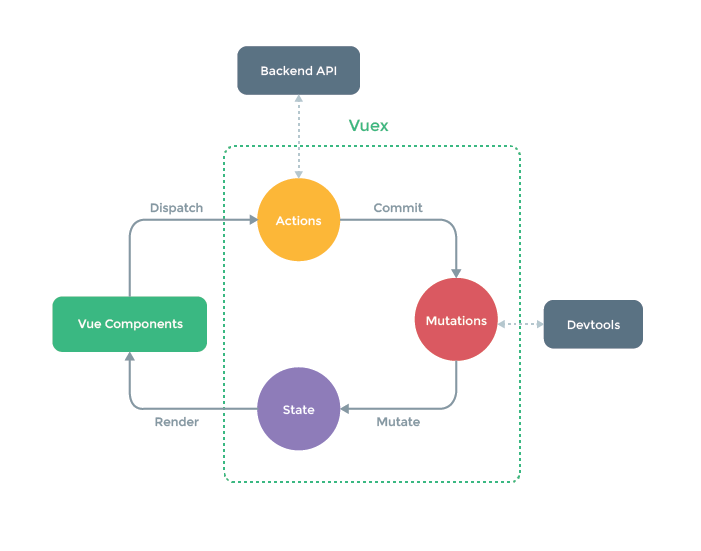
\includegraphics[width=\textwidth]{figures/vuex}
\caption{Schemat przepływu danych w Vuex.}\label{rys:vuex}
\end{figure}

\subsection{Jest}
W projekcie wykorzystano framework testowy Jest będący częścią Vue Test Utils. Vue Test Utils to zestaw funkcjonalności upraszczających testowanie komponentów Vue.js. Zestaw ten zapewnia metody umożliwiające symulowanie działań użytkownika w aplikacji oraz przechwytywanie i porównywanie rezultatów tych interakcji z oczekiwanymi. Jest cechuje brak konieczności konfiguracji, izolacja testów oraz szybkość i bezpieczeństwo działania.
\subsection{Json Web Tokens}
Json Web Token jest otwartym standardem przesyłania zabezpieczonych danych. Dane w formacie Json są podpisywane cyfrowo co umożliwia weryfikacje uprawnień. W aplikacjach internetowych JWT stosowane są głownie do autoryzacji użytkowników oraz zapewnienia bezpieczeństwa przesyłanie informacji pomiędzy frotendem, a backendem. Niewielki rozmiar tokenu sprawia iż możliwe jest przesyłanie go w treści zapytania HTTP lub nawet w jego nagłówku. Ta cecha sprawia również, że token może być przechowywany w pamięci przeglądarki, eliminując konieczność ponownego uwierzytelniania po rozpoczęciu nowej sesji.
\subsection{Postman}
Postman jest zestawem narzędzi do testowania API (application programming interface). Zapewnia on możliwość wysyłania zapytań HTTP dowolnego typu oraz podgląd odpowiedzi i kodów błędów, jeśli takie wystąpiły. Główną zaletą Postmana jest możliwość tworzenia kolekcji zapytań, które ułatwiają organizację pracy podczas planowania połączeń pomiędzy częścią frontendową i backendową aplikacji. Dodatkowo narzędzie pozwala na współdzielenie kolekcji z zaproszonymi użytkownikami, co znacząco upraszcza proces testowania manualnego. Poza testowaniem manualnym Postman umożliwia tworzenie automatycznych testów przy pomocy języka JavaScript. Dzięki generatorowi losowych danych możliwa jest symulacja działań nawet kilku tysięcy różnych użytkowników w systemie.
\subsection{Visual Studio Code}
Visual Studio Code jest edytorem kodu, którego głównymi zaletami jest wsparcie dla debugowania, inteligentnego uzupełniania kodu, refaktoryzacji oraz kontroli wersji. Dużą korzyścią płynącą z korzystania z program Visual Studio Code jest dostęp do rozszerzeń, usprawniających pracę z kodem w dowolnym języku programowania. Rozszerzenia zapewniają również wsparcie dla frameworków, w tym Vue.js, najbardziej istotnym dla tej części projektu. Mały rozmiar oraz wysoka wydajność znacznie przyśpieszają korzystanie z aplikacji i sprzyjają intensywnej iteracji rozwiązań.
\subsection{Axios}
Axios jest biblioteką języka JavaScript służąca do wykonywania zapytań HTTP z poziomu Node.js lub przeglądarki. W aplikacjach internetowych wykorzystywany jest do uzyskiwania danych z części backendowej aplikacji. Axios bazuje na obietnicach (promise), co pozwala na obsługiwanie akcji asynchronicznie. Biblioteka może być użyta poprzez zwykły Javascript lub framework taki jak Vue.js. W porównaniu z innymi bibliotekami służącymi do wykonywania zapytań HTTP Axios oferuje wsparcie dla starszych przeglądarek, możliwość ustawienia ograniczenia czasowego dla zapytań, ochronę przed CSRF (Cross-Site Request Forgery), a także automatyczną transformację danych JSON.
\subsection{Bootstrap}
Bootstrap jest frameworkiem CSS (Cascading Style Sheets) upraszczającym projektowanie interfejsu graficznego aplikacji internetowych. Bootstrap pomaga zapewnić responsywność stron, a więc poprawne ich wyświetlanie na urządzeniach mobilnych. Przed pojawieniem się tego rozwiązania często występowała konieczność przygotowywania oddzielnych stylów dla ekranów o rożnych rozdzielczościach. Dzięki zastosowaniu frameworku elementy strony internetowe zostają przeskalowane i przemieszczone tak, aby pomieścić się na ekranie niezależnie od jego wielkości i proporcji. Dodatkowo Bootstrap pozwala na zastosowanie zaawansowanych komponentów takich jak paski nawigacji, wskaźniki postępu czy miniatury. 

\clearpage
\section{Widoki}
\subsection{Strona główna}
Strona główna aplikacji została stworzona na bazie szablonu Bootstrap o nazwie One Page Wonder(źródło). Zawiera ona krótki opis aplikacji, a także korzyści płynących z wykorzystania jej dla planistów, nauczycieli oraz uczniów. Pasek menu znajdujący się zawsze na górze strony jest stałym elementem aplikacji pojawiającym się w każdym z widoków. Pozwala on na przejście do widoków logowania i rejestracji, a przypadku gdy użytkownik jest już zalogowany na wylogowanie lub przejście do widoku szkoły. 
\begin{figure}[!ht]
\centering
\includegraphics[width=\textwidth]{figures/main}
\caption{Aplikacja internetowa - Strona głowna}\label{rys:main}
\end{figure}
\subsection{Widok szkoły}
Widok szkoły pozwala na przejście do dodawania danych potrzebnych do wygenerowania planu, a przypadku gdy plan został już wygenerowany jest również miejscem w którym jest on wyświetlany. Rozkład zajęć jest możliwy do wyświetlenia na trzy sposoby - z podziałem na klasy, nauczycieli lub sale lekcyjne.

\begin{figure}[!ht]
\centering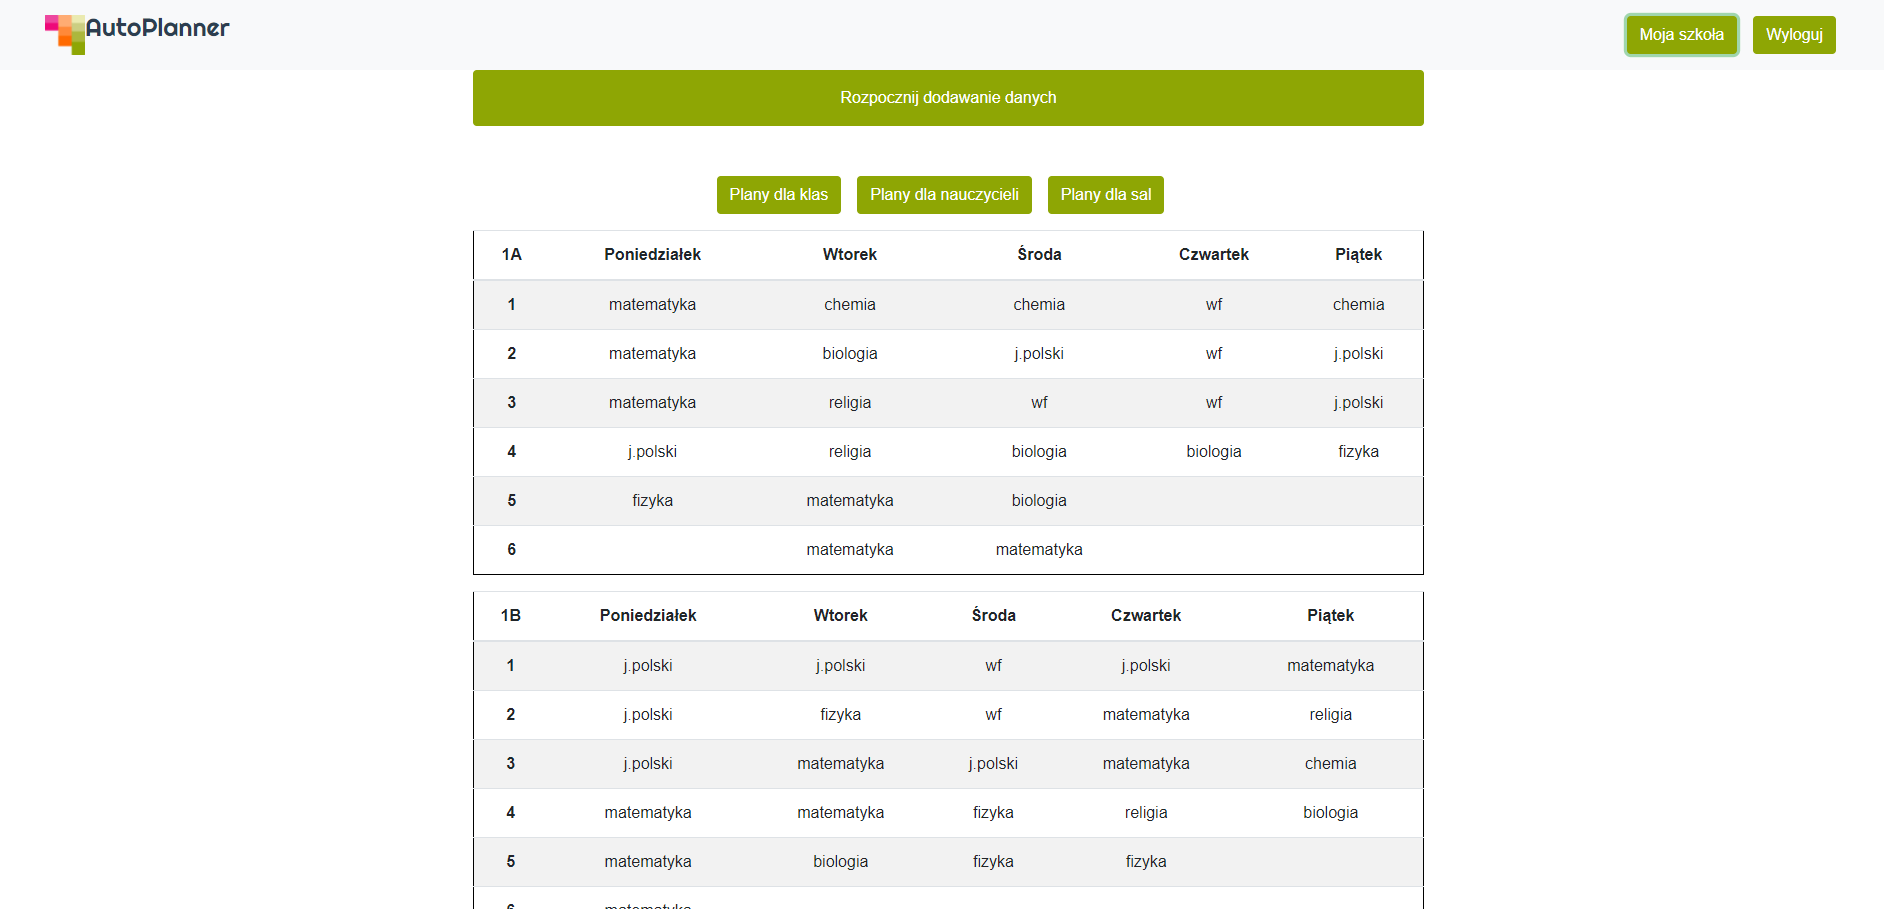
\includegraphics[width=\textwidth]{figures/school}
\caption{Aplikacja internetowa - Widok szkoły}\label{rys:school}
\end{figure}
\subsection{Rejestracja}
Widok rejestracji umożliwia utworzenie konta w serwisie. Od użytkownika wymaga się podania adresu e-mail, nazwy użytkownika oraz hasła. Adres e-mail musi być unikatowy. Wynika to z konieczności weryfikacji konta poprzez wiadomość wysłaną przy pomocy serwera SMTP. Rozwiązanie to ma na celu zapobieganie atakom na stronę poprzez masowe tworzenie nowych kont. 
\begin{figure}[!ht]
\centering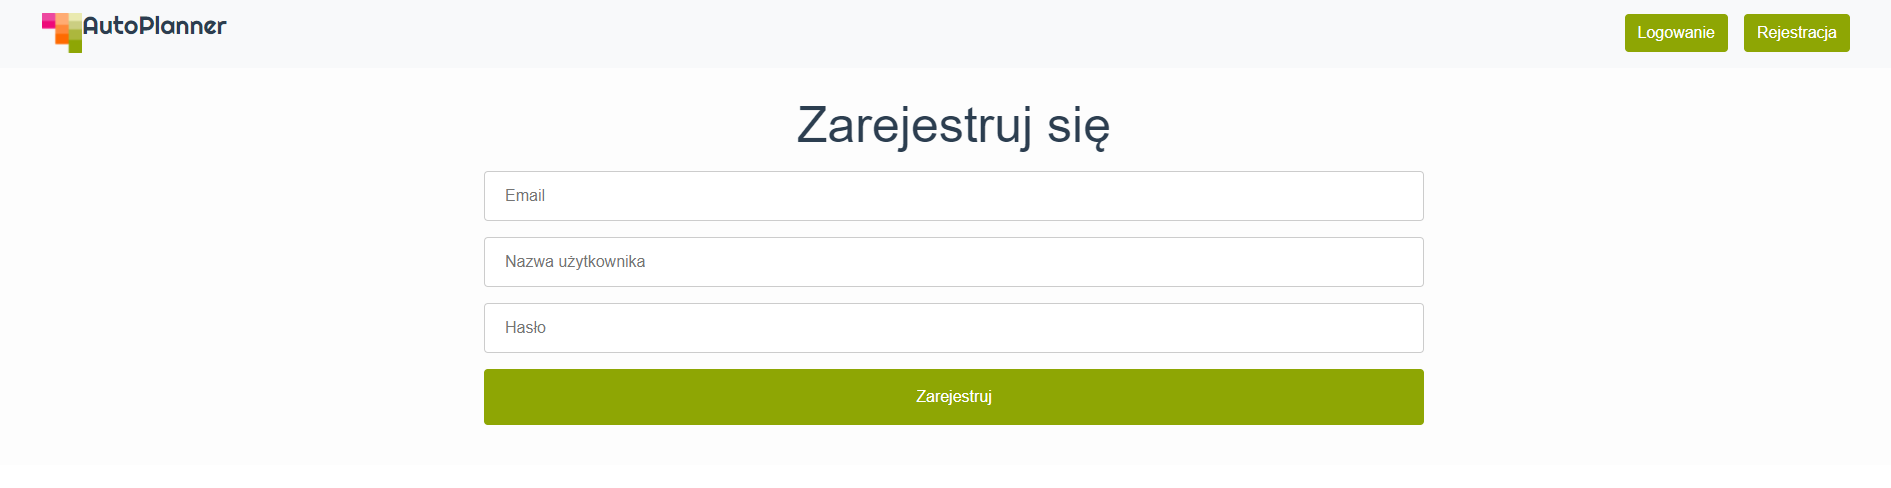
\includegraphics[width=\textwidth]{figures/register}
\caption{Aplikacja internetowa - Widok rejestracji}\label{rys:register}
\end{figure}
\subsection{Logowanie}
Widok logowania pozwala na dostęp do konta i zapisanych na nim danych z dowolnego urządzenia. Do uwierzytelnienia użytkownika wykorzystywany jest adres e-mail oraz hasło podane w procesie rejestracji. Powodzenie procesu logowania powoduje otrzymanie przez aplikację tokenu JWT, zapisywanego w pamięci przeglądarki. W przypadku utraty hasła użytkownik posiada możliwość odzyskania go po podaniu adresu e-mail powiązanego z istniejącym kontem.
\begin{figure}[!ht]
\centering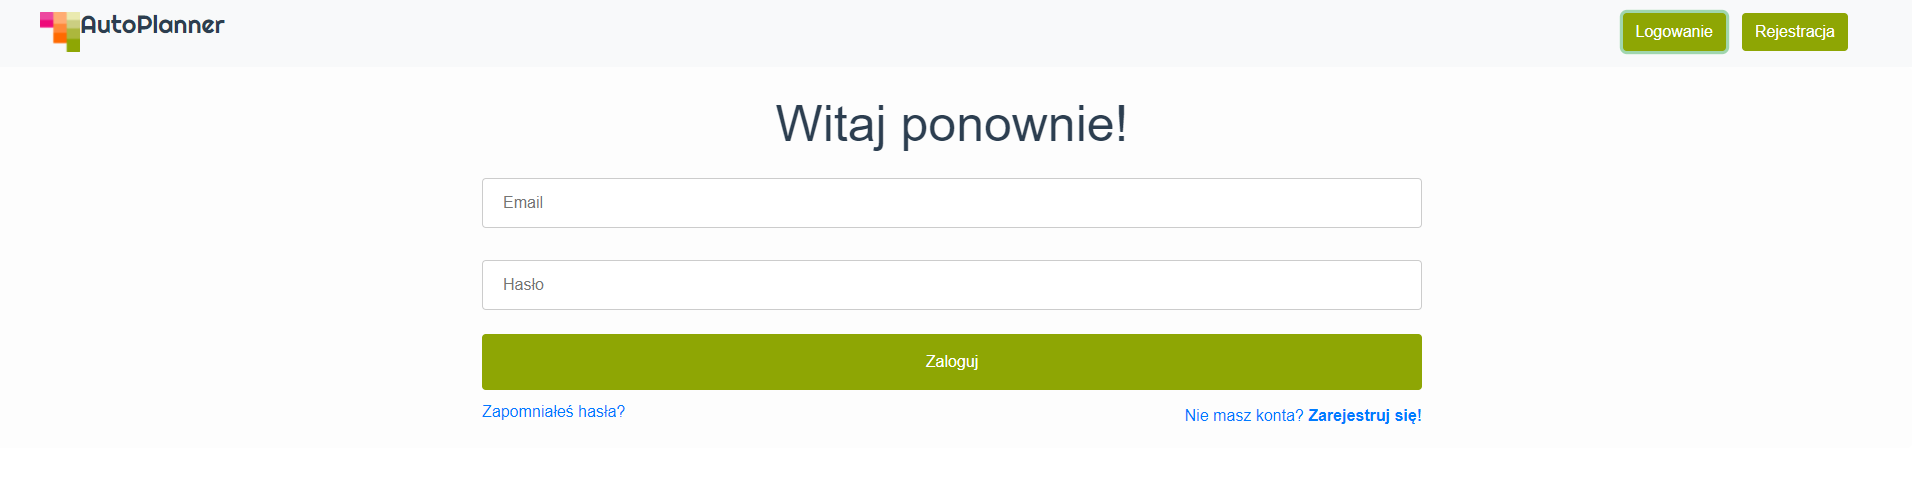
\includegraphics[width=\textwidth]{figures/login}
\caption{Aplikacja internetowa - Widok logowania}\label{rys:login}
\end{figure}
\clearpage
\subsection{Ankieta}
Widok ankiety pozwala nauczycielowi na podanie preferencji godzinowych pracy. W przeciwieństwie do pozostałych widoków jest on dostępny jedynie poprzez bezpośredni link wysyłany w wiadomości e-mail. Takie rozwiązanie sprawia, że jedynym użytkownikiem, od którego wymagane jest posiadanie konta jest planista. Nauczyciele jako użytkownicy bez konta są identyfikowani dzięki unikalności adresu URL.
\begin{figure}[!ht]
\centering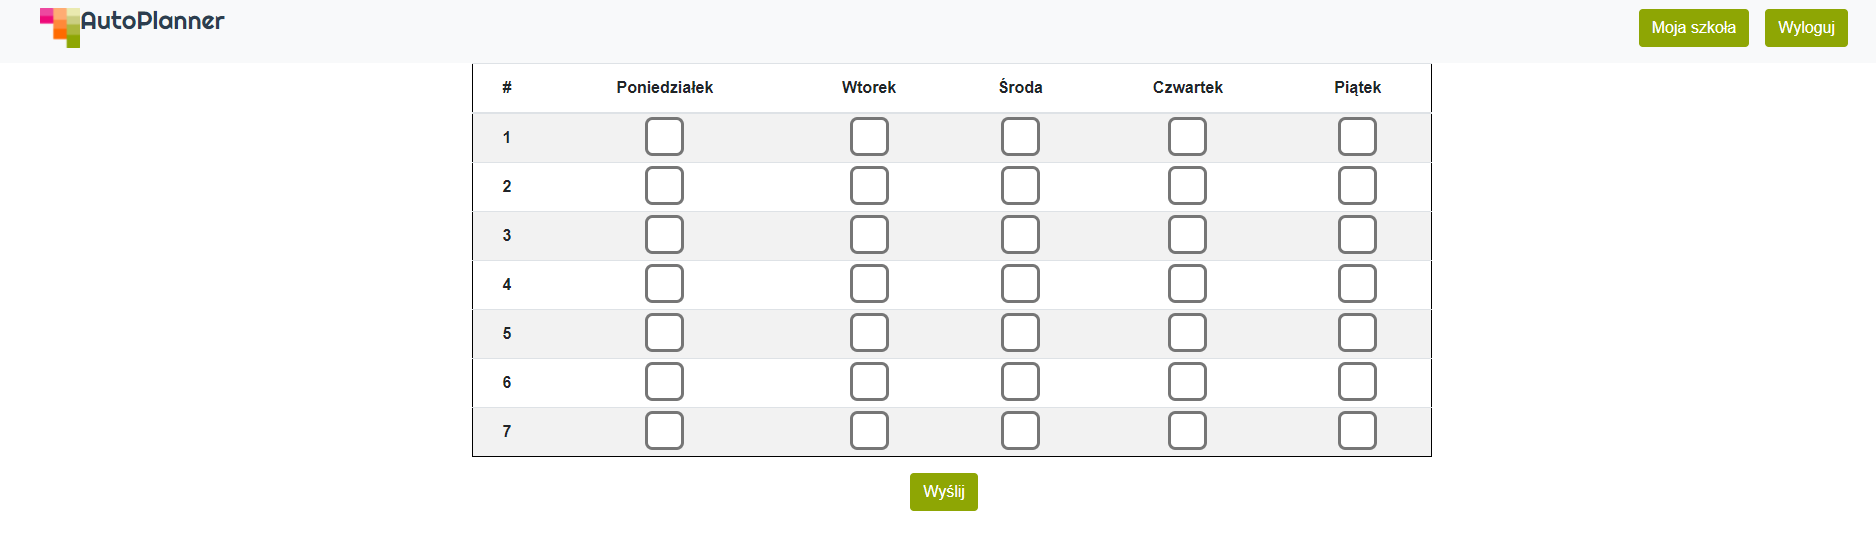
\includegraphics[width=\textwidth]{figures/poll}
\caption{Aplikacja internetowa - Widok ankiet dla nauczycieli}\label{rys:poll}
\end{figure}
\subsection{Dodawanie przedmiotów}
Widok dodawania przedmiotów stanowi pierwszy krok w procesie podawania danych koniecznych do wygenerowania planu zajęć. W celu dodawania przedmiotu należy podać jedynie jego nazwę. Powiązania z nauczycielami, salami lekcyjnymi i klasami będą mogły być wprowadzone w kolejnych krokach. Podanie nazw przedmiotów na początku procesu dodawania danych pozwala na to, aby w późniejszych etapach mogły być one wybierane z listy rozwijanej. Zapobiega to konieczności wielokrotnego ręcznego wprowadzania tych samych informacji i ułatwia tworzenie powiązań w bazie danych. W lewej części ekranu znajduje się lista już wprowadzonych przedmiotów. Wybranie z nich jednego powoduje przejście do ekranu edycji. Analogiczne rozwiązanie zostało zastosowane we wszystkich kolejnych ekranach dodawania danych.
\begin{figure}[!ht]
\centering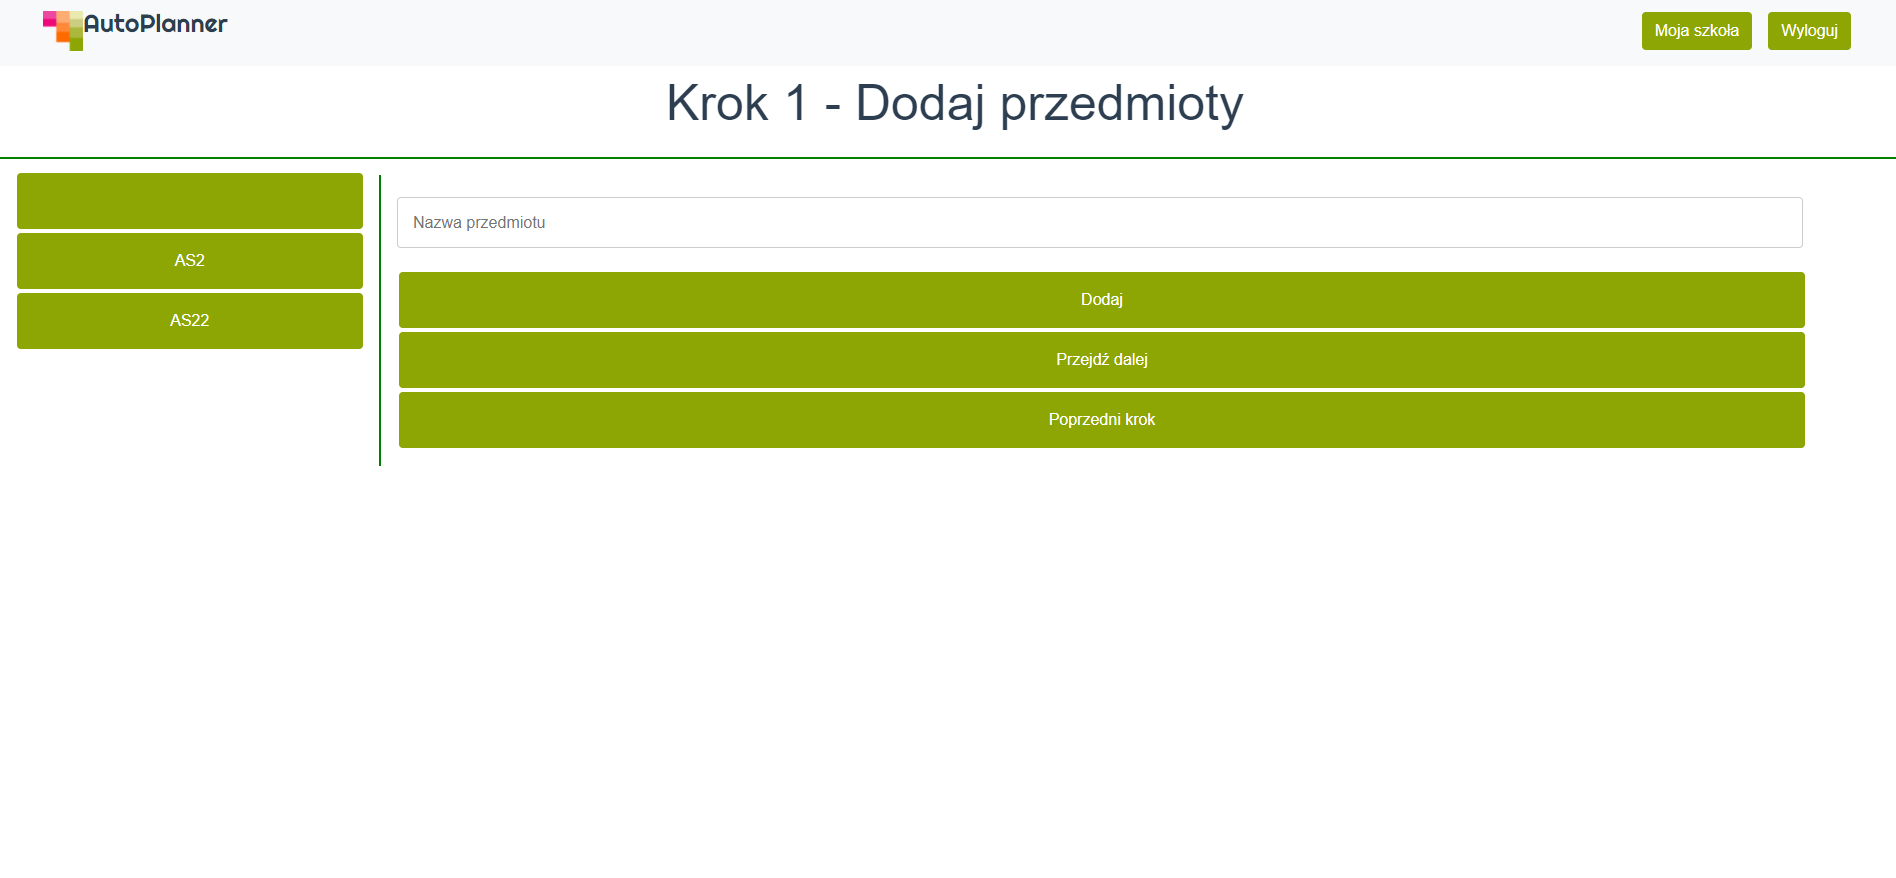
\includegraphics[width=\textwidth]{figures/subject}
\caption{Aplikacja internetowa - Widok dodawania przedmiotów}\label{rys:subject}
\end{figure}
\subsection{Dodawanie nauczycieli}
W widoku dodawania nauczycieli planista ma możliwość wprowadzenia danych personelu dydaktycznego oraz jego powiązań z przedmiotami. Każdy nauczyciel musi posiadać imię i nazwisko, unikalny w skali szkoły adres e-mail oraz przynajmniej jeden prowadzony przedmiot. Ekran umożliwia dodanie kolejnych prowadzonych przedmiotów w przypadku, gdy nauczyciel prowadzi więcej niż jeden. 
\begin{figure}[!ht]
\centering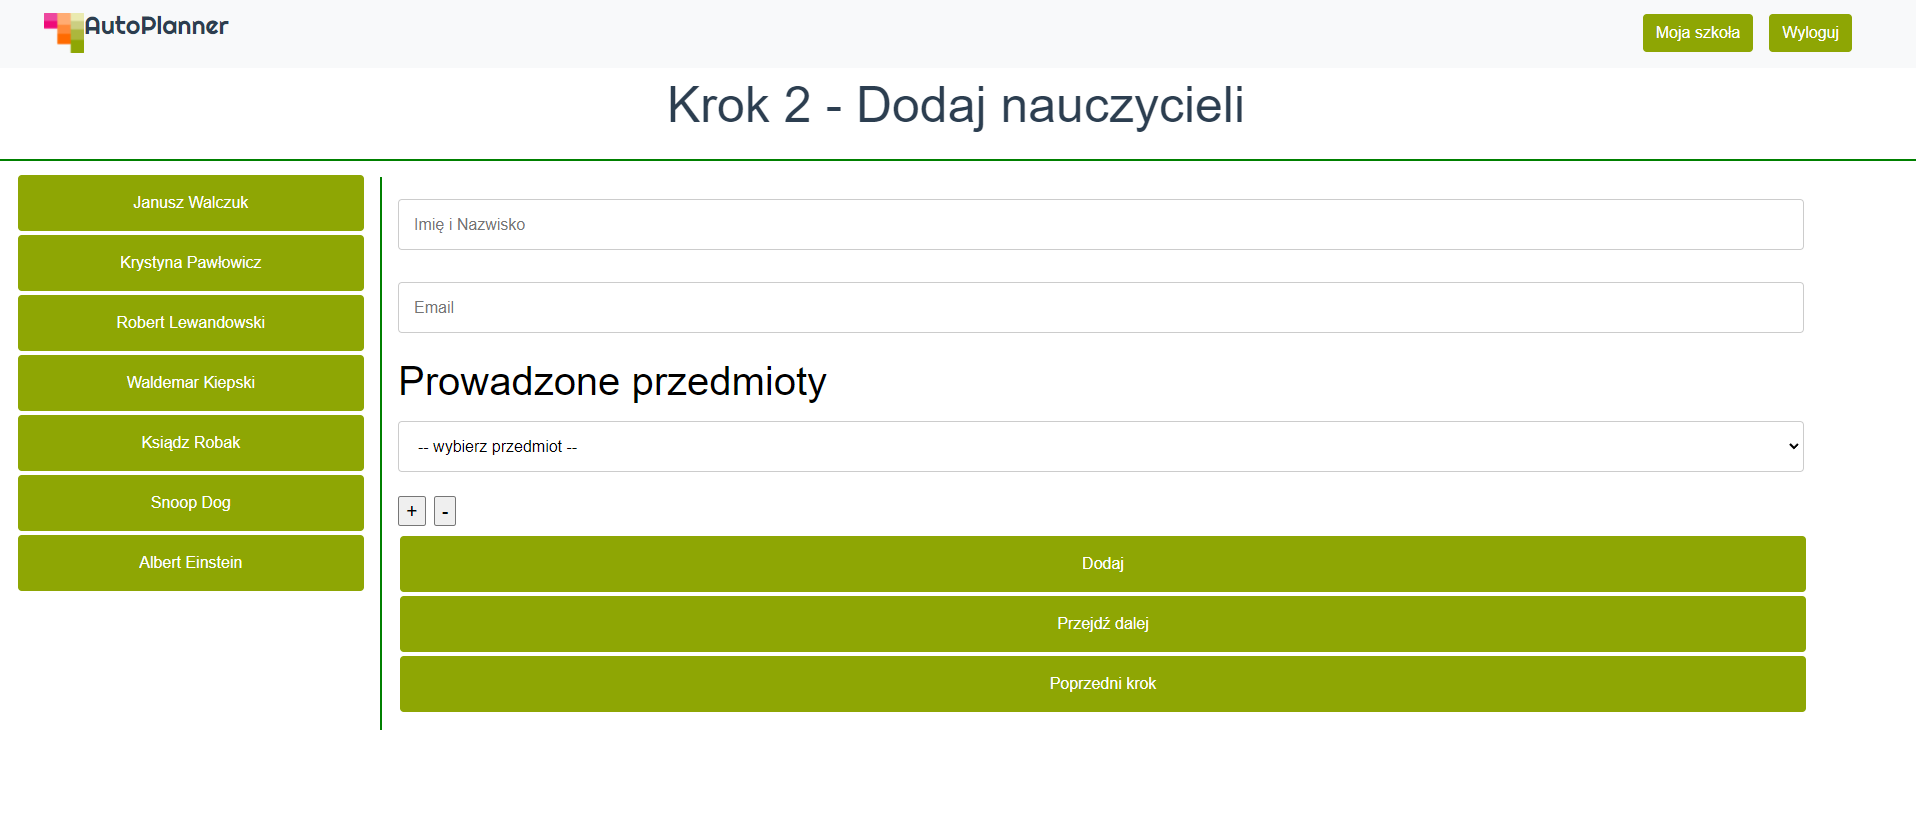
\includegraphics[width=\textwidth]{figures/teacher}
\caption{Aplikacja internetowa - Widok dodawania nauczycieli}\label{rys:teacher}
\end{figure}
\subsection{Dodawanie sali lekcyjnych}
Dodanie informacji o salach lekcyjnych stanowi trzeci krok dodawania danych. Sala lekcyjna musi posiadać nazwę, a opcjonalnie także listę przedmiotów, które mogą być w  niej prowadzone. W przypadku, gdy nie zostanie wybrany żaden preferowany przedmiot sala zostaje uznana za salę zwykłą, co oznacza, że będzie mógł być w niej prowadzony dowolny przedmiot.
\begin{figure}[!ht]
\centering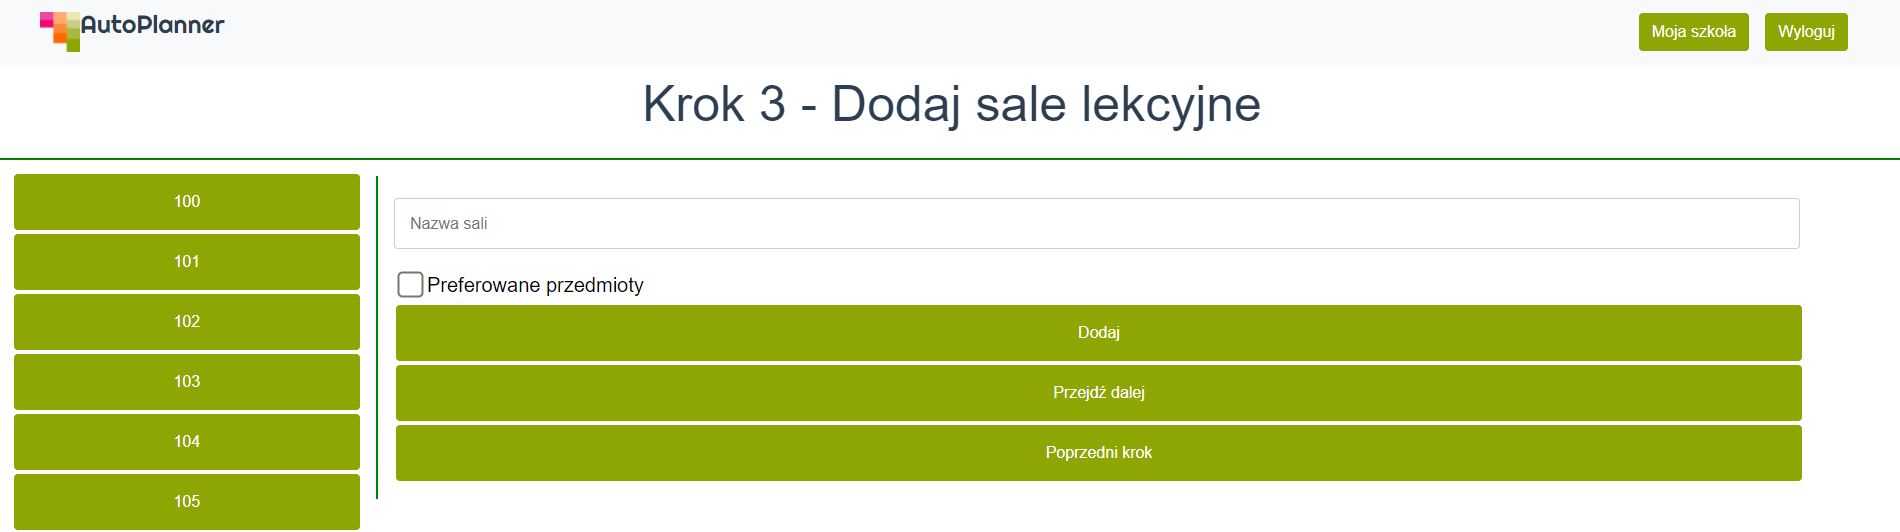
\includegraphics[width=\textwidth]{figures/classroom}
\caption{Aplikacja internetowa - Widok dodawania sali lekcyjnych}\label{rys:classroom}
\end{figure}
\subsection{Dodawanie klas}
Ostatnim etapem w procesie dodawania niezbędnych danych jest wprowadzenie parametrów klas. Każda klasa musi posiadać nazwę oraz listę przedmiotów, które mają się pojawić w jej planie zajęć. Każdy element listy musi zawierać nazwę przedmiotu, liczbę godzin lekcyjnych w tygodniu przeznaczonych na przedmiot oraz opcjonalnie prowadzącego przedmiot. Brak wyboru nauczyciela umożliwia przypisanie zajęć dowolnemu prowadzącemu dany przedmiot.
\begin{figure}[!ht]
\centering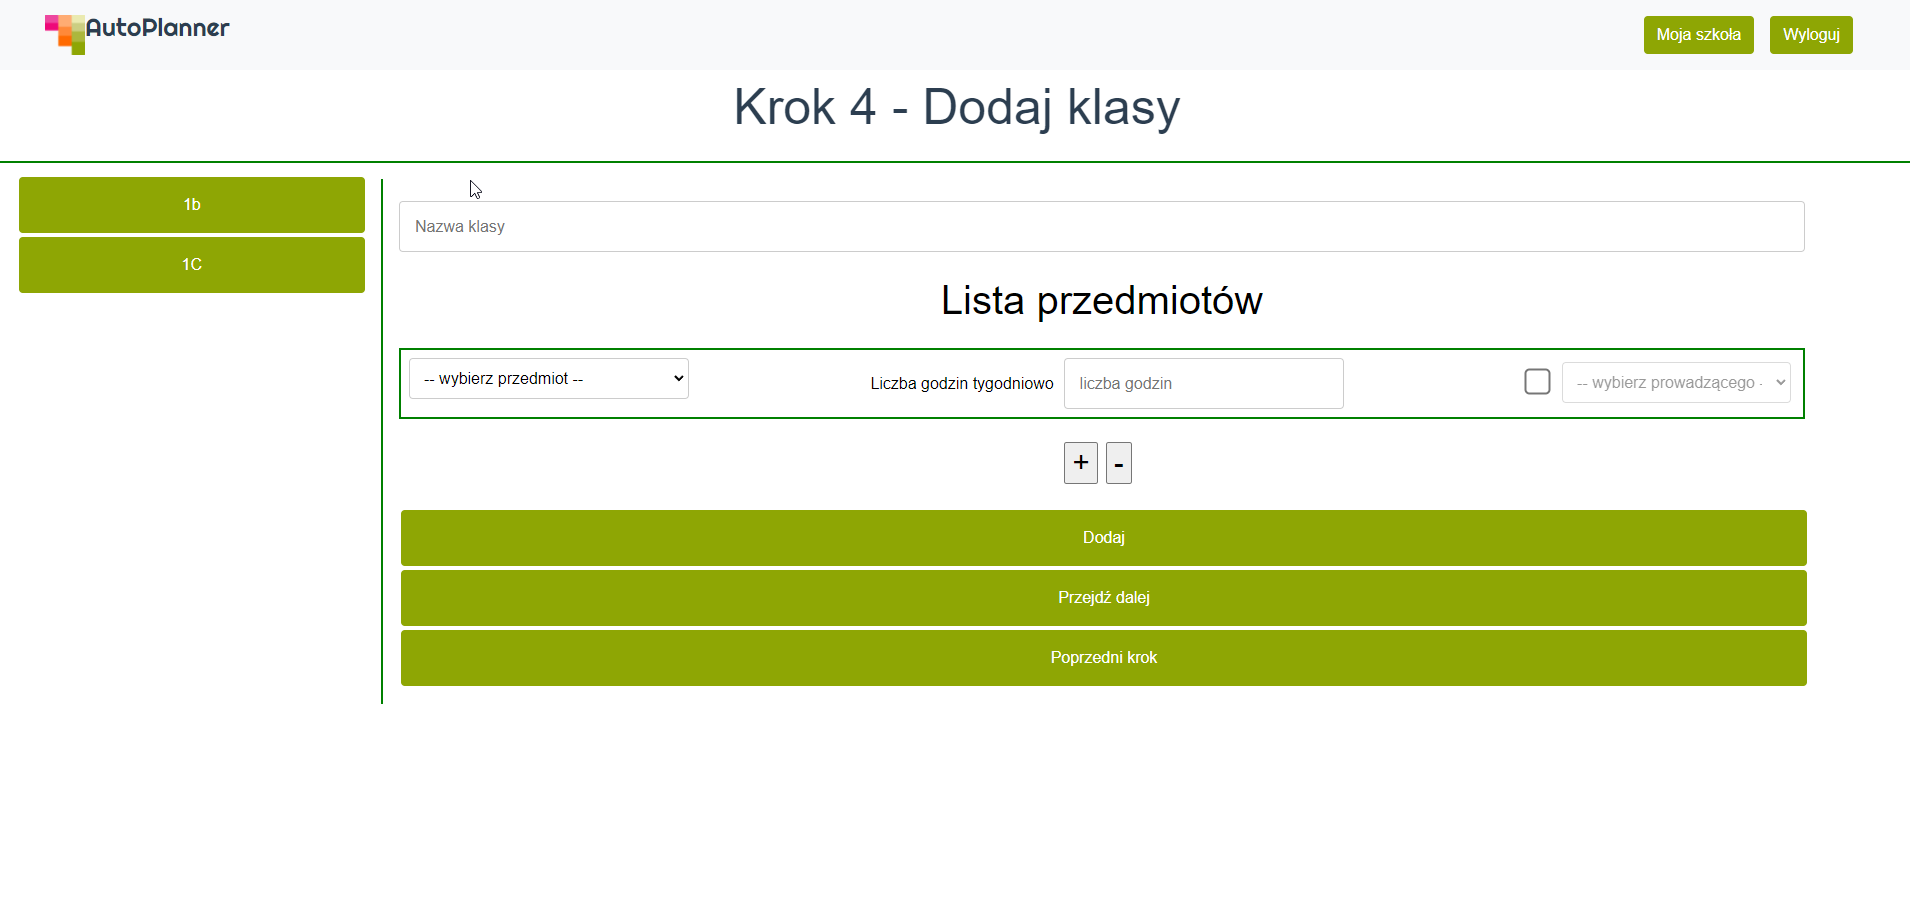
\includegraphics[width=\textwidth]{figures/class}
\caption{Aplikacja internetowa - Widok dodawania klas}\label{rys:class}
\end{figure}
\subsection{Edycja danych}
Dla czterech powyższych ekranów istnieją odpowiadające im ekrany edycji danych. Ze względu na ich analogiczną budowę omówiony zostanie ich struktura zostanie omówiona na bazie widoku edycji danych nauczyciela. Przejście do tego ekranu umożliwiają przyciski znajdujące się po prawej stronie widoku dodawania nauczycieli. Przyciski te są wciąż obecne w widoku edycji i pozwalają na przechodzenie pomiędzy danymi poszczególnych osób bez zapisywania wprowadzonych zmian. W chwili przejścia do ekranu edycji pola z danymi zostają uzupełnione pierwotnie wprowadzonymi informacjami o nauczycielu. Takie rozwiązanie ma celu zapobieganie konieczności ponownego wprowadzania wszystkich danych, w przypadku gdy tylko niektóre z nich wymagają zmian. Przyciski u dołu pozwalają na zapisanie wprowadzonych zmian, powrót do ekranu dodawania nauczycieli lub całkowite usunięcie nauczyciela z bazy danych.
\begin{figure}[!ht]
\centering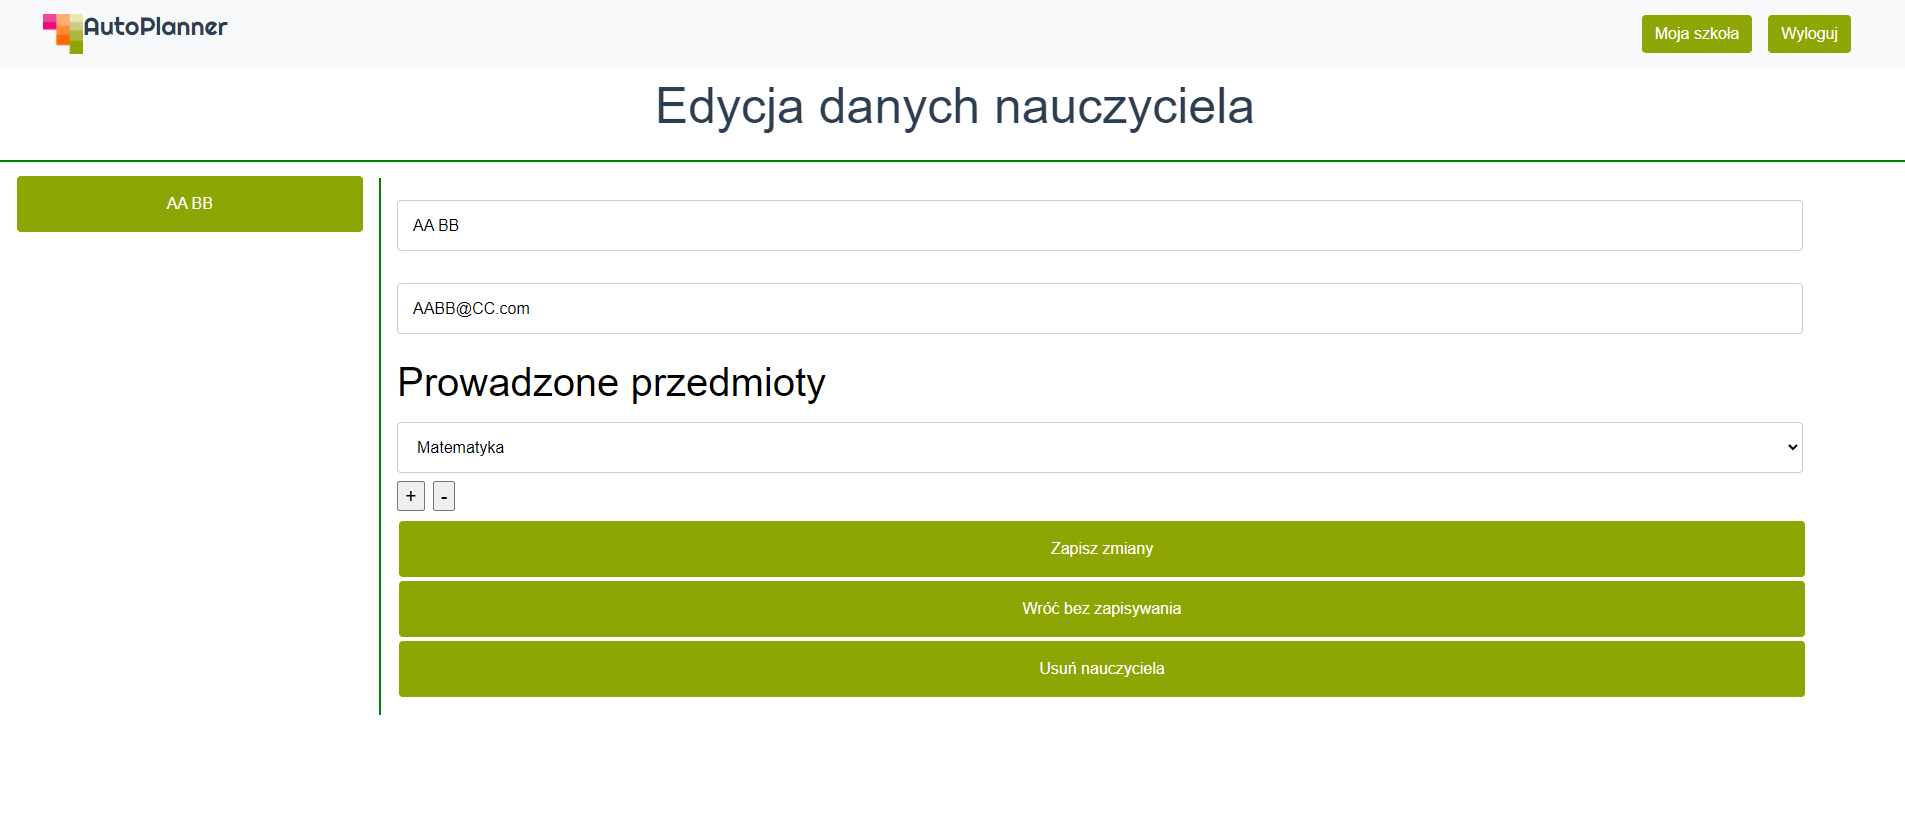
\includegraphics[width=\textwidth]{figures/edit}
\caption{Aplikacja internetowa - Widok edycji danych nauczyciela}\label{rys:edit}
\end{figure}






\chapter{Projekt i implementacja strony serwerowej opartej na architekturze REST w technologi Django oraz bazy danych MySQL}
\section{Narzędzia i techonologie}
\subsection{Django}
Django~\cite{Django} jest darmową, wysoko poziomową platformą programistyczną przeznaczoną do tworzenia aplikacji internetowych. Dostarcza wiele narzędzi ułatwiających szybką oraz prostą implementacje. Oparta jest na wzorcu architektonicznym model-template-view. ~\ref{rys:django} Napisana jest w języku Python. Jednymi z najważniejszych cech Django są:
\begin{itemize}
	\item Łatwy i bezpieczny dostęp do bazy danych
	\item Duża skalowalność oraz wydajność
	\item Wbudowane zabezpieczenia przed popularnymi atakami
	\item Rozbudowana dokumentacja
\end{itemize}
\begin{figure}[H]
	\centering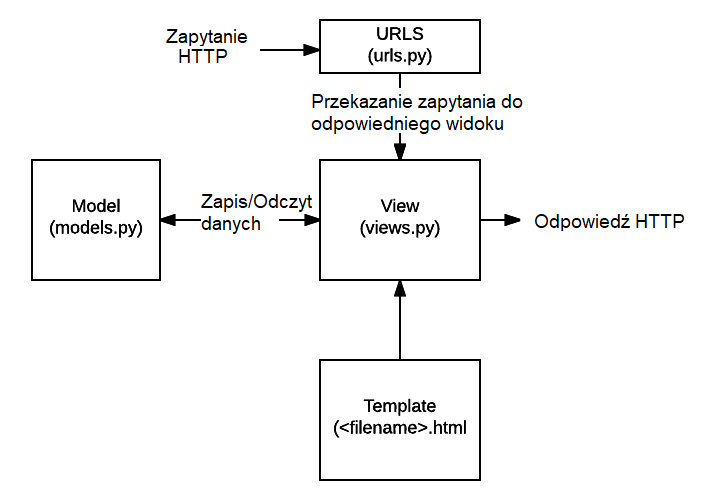
\includegraphics[width=\textwidth]{figures/DjangoSchemat}
	\caption{Schemat przepływu danych w Django~\cite{DjangoSchemat}}\label{rys:django}
\end{figure}
\subsection{MySQL}
MySQL~\cite{SQL} jest systemem służącym do zarządzania relacyjnymi bazami danych. Model relacyjny zapewnia łatwość w projektowaniu oraz implementacji. Udostępniony jest na licencji wolnego oprogramowania i dostępny jest dla wszystkich popularnych systemów operacyjnych. Bazy danych oparte na tym systemie są wstanie obsługiwać olbrzymie ilości zapytań w bardzo krótkim czasie.
\subsection{MySQL Workbench}
MySQL Workbench~\cite{Workbench} to narzędzie do projektowania, tworzenia oraz zarządzania bazami danych MySQL. Posiada bardzo przejrzysty i intuicyjny interfejs, przez co cieszy się dużą popularnością. Wiele podstawowych czynności takich jak np. tworzenie i edycja tabel, można wykonać bez znajomości zapytań SQL, gdyż są one generowane automatycznie.

\section{Implementacja serwera REST API}
\subsection{REST}
REST ~\cite{REST} jest stylem architektonicznym wprowadzającym pewien standard komunikacyjny dla internetowych systemów informatycznych. Jego najważniejszymi zaletami są szybkość oraz uniwersalność. Interfejsy programistyczne spełniające założenia REST mogą komunikować się dowolnym urządzeniem sieciowym, pod warunkiem wysyłania przez nie zapytań w odpowiednim formacie. Jednymi z głównych zasad tego stylu są:
\begin{itemize}
	\item Zastosowanie modelu klient-serwer
	\item Bezstanowość
	\item Wykorzystywanie pamięci cache przeglądarki w celu zapamiętywania odpowiedzi
	\item Interfejs programistyczny jednolity dla każdej aplikacji klienckiej
\end{itemize}
\begin{figure}[H]
	\centering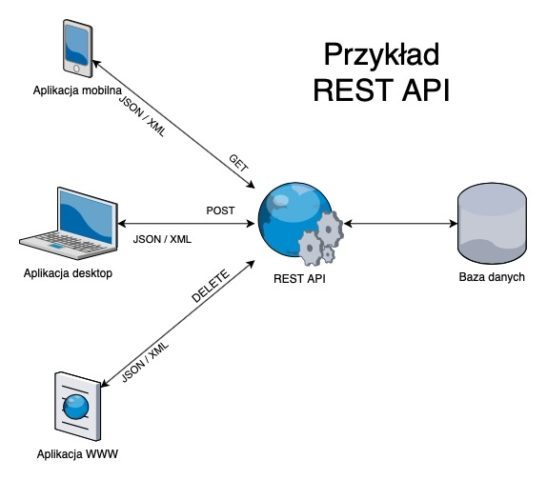
\includegraphics[width=\textwidth]{figures/rest}
	\caption{Przykładowy schemat działania REST API~\cite{SchematRest}}\label{rys:rest}
\end{figure}

Zapytania zazwyczaj wysyłane są przy pomocy protokołu HTTP. Zarówno do zapytań, jak i do odpowiedzi, najczęściej wykorzystywane są metody GET oraz POST. Informacje przesyłane między klientem a serwerem muszą być precyzyjne, zwykle występują one w formacie JSON. 

\subsection{Modele}
Jednym z najważniejszych mechanizmów zaimplementowanych w Django są Modele. Są one swego rodzaju mapowaniem klas języka Python na tabele bazy danych. Takie rozwiązanie zapewnia bardzo szybki i wygodny dostęp do przechowywanych informacji. Klasy te zdefiniowane są w pliku "models.py". Wykorzystując wbudowane funkcje wykorzystywanej platformy programistycznej, możemy zarówno wygenerować tabele bazy danych na podstawie modeli, jak i wygenerować modele na podstawie gotowych tabel.

W projekcie znajduje się następujące siedem modeli: 
\begin{itemize}
	\item Classrooms
	\item Lessons
	\item Planners
	\item Polls
	\item Subjects
	\item Teachers
	\item Timetables
\end{itemize}
Każdy odpowiada jednej tabeli z bazy danych, pola w każdej z klas są analogiczne do kolumn w odpowiednich tabelach. Zawierają informacje takie jak mp. typ danych, maksymalna długość oraz co jest kluczem głównym.
Implementacja przykładowej klasy:
\begin{figure}[H]
	\centering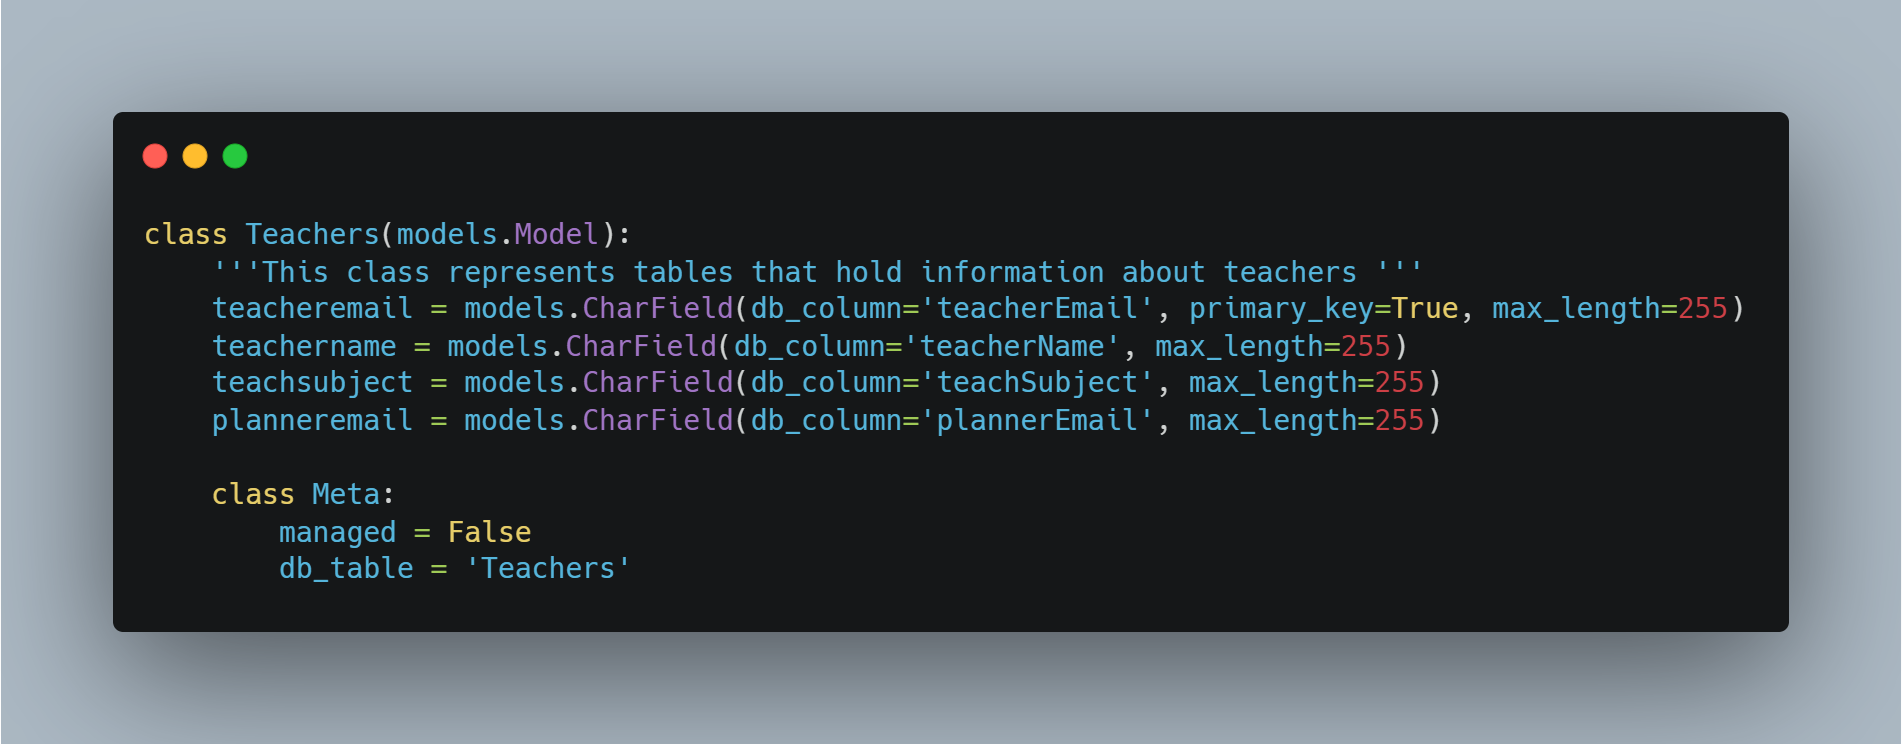
\includegraphics[width=\textwidth]{figures/TeachersModel}
	\caption{Implementacja klasy Teachers}\label{rys:TeachersModel}
\end{figure}

\subsection{Adresy internetowe}
Kolejnym elementem implementacji są adresy internetowe. W pliku "urls.py" określone zostały wykorzystywane w projekcie adresy URL, oraz funkcje które mają zostać wywołane w przypadku otrzymania od klienta zapytania na dany adres. Implementacja przedstawiona na rysunku ~\ref{rys:URLs}
\begin{figure}[H]
 	\centering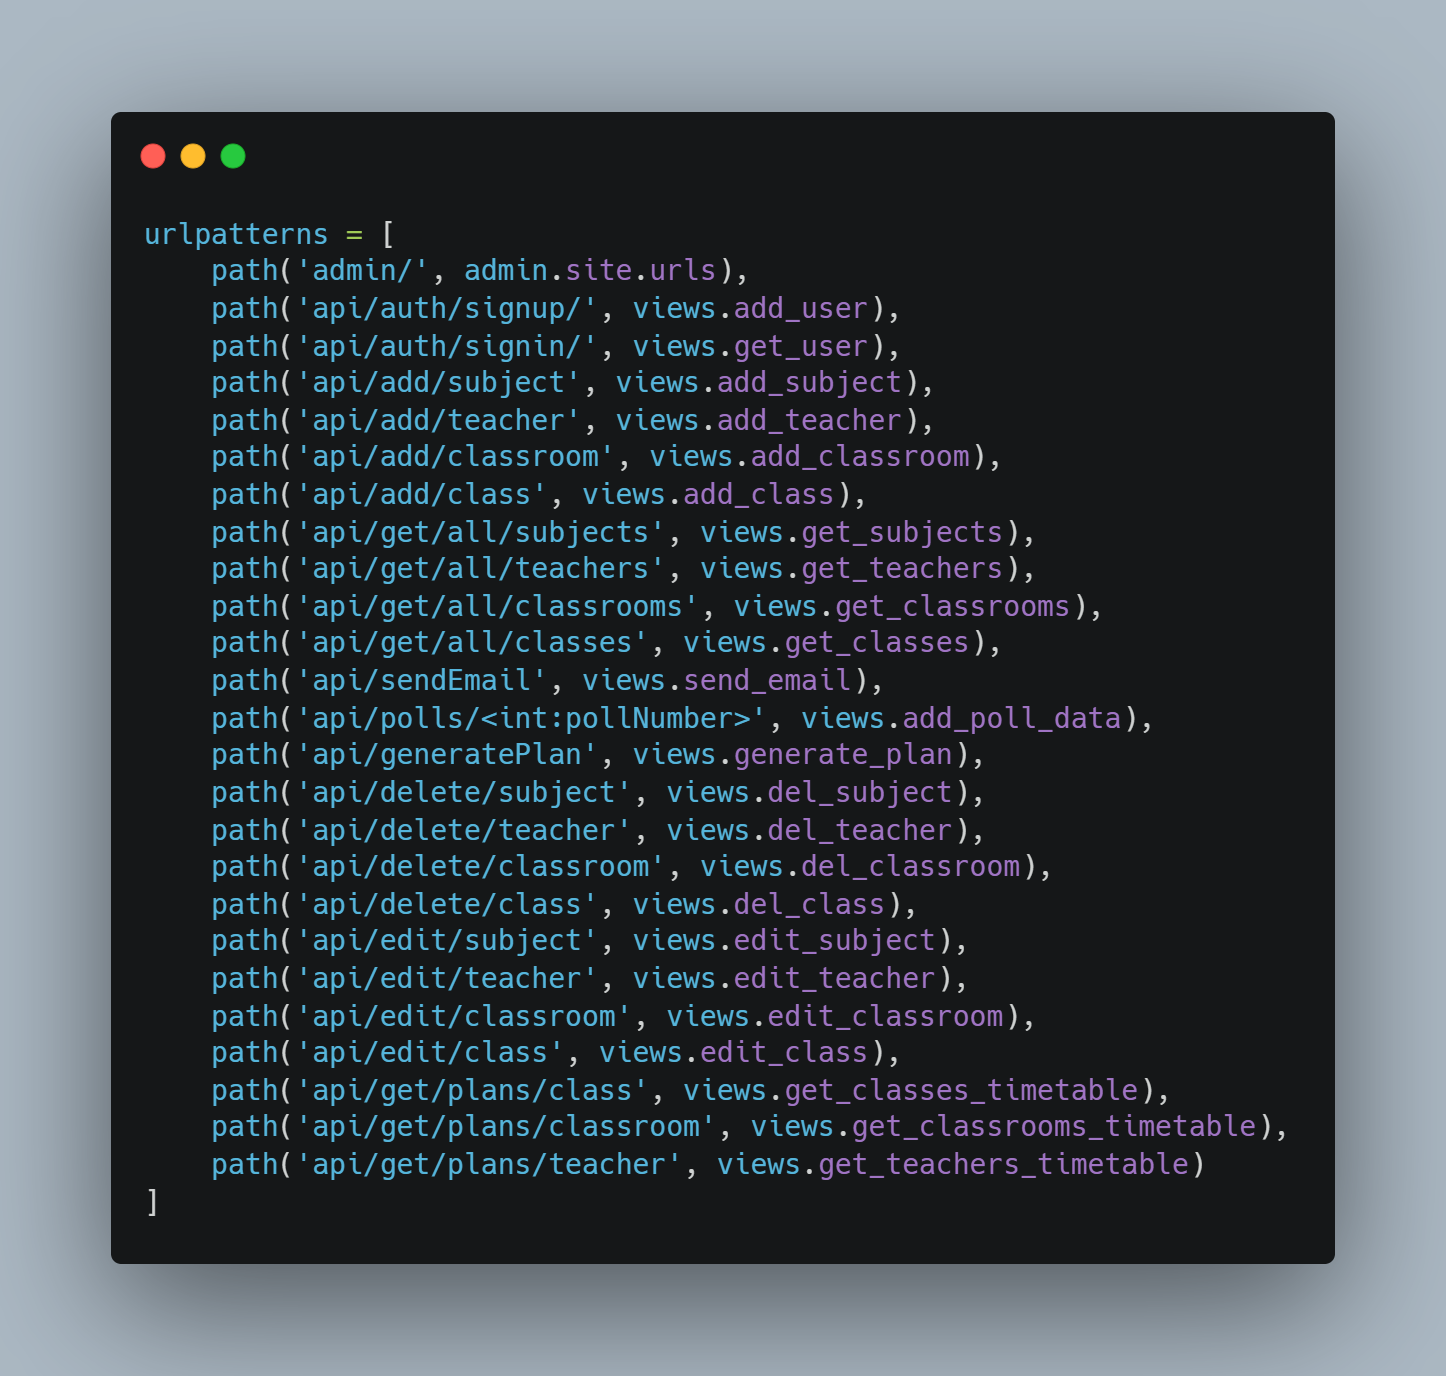
\includegraphics[width=\textwidth]{figures/Urls}
 	\caption{Implementacja adresów URL}\label{rys:URLs}
\end{figure}
W przypadku, jeśli zapytanie przyjdzie na niezadeklarowany adres, zwrócony zostanie komunikat HTTP z kodem 404(Page Not Found).

\subsection{Widoki}
Widoki to nic innego, jak funkcję języka python wykonywane w momencie odbioru zapytania przez serwer. Kiedy klient wyśle zapytanie na dany adres, django sprawdza czy jest on zadeklarowany we wspomnianym wcześniej pliku "urls.py", jeśli tak, to wywoływana jest odpowiednia funkcja z pliku "views.py" wraz z jej parametrem którym jest samo zapytanie. Dzięki takiej parametryzacji, widok ma łatwy dostęp do otrzymanych informacji, sprawdza on czy są one prawidłowe, oraz wykonuje na nich odpowiednie działania. W tym projekcie, w większości przypadków wykonywane są operacje zapisu i odczytu z bazy danych. Do komunikacji wykorzystywane są metody GET oraz POST z protokołu HTTP.
Implementacje przykładowych widoków obsługujacych zapytania dla danych metod HTTP na rysunkach ~\ref{rys:BackendGet} oraz ~\ref{rys:BackendPost}
\begin{figure}[H]
	\centering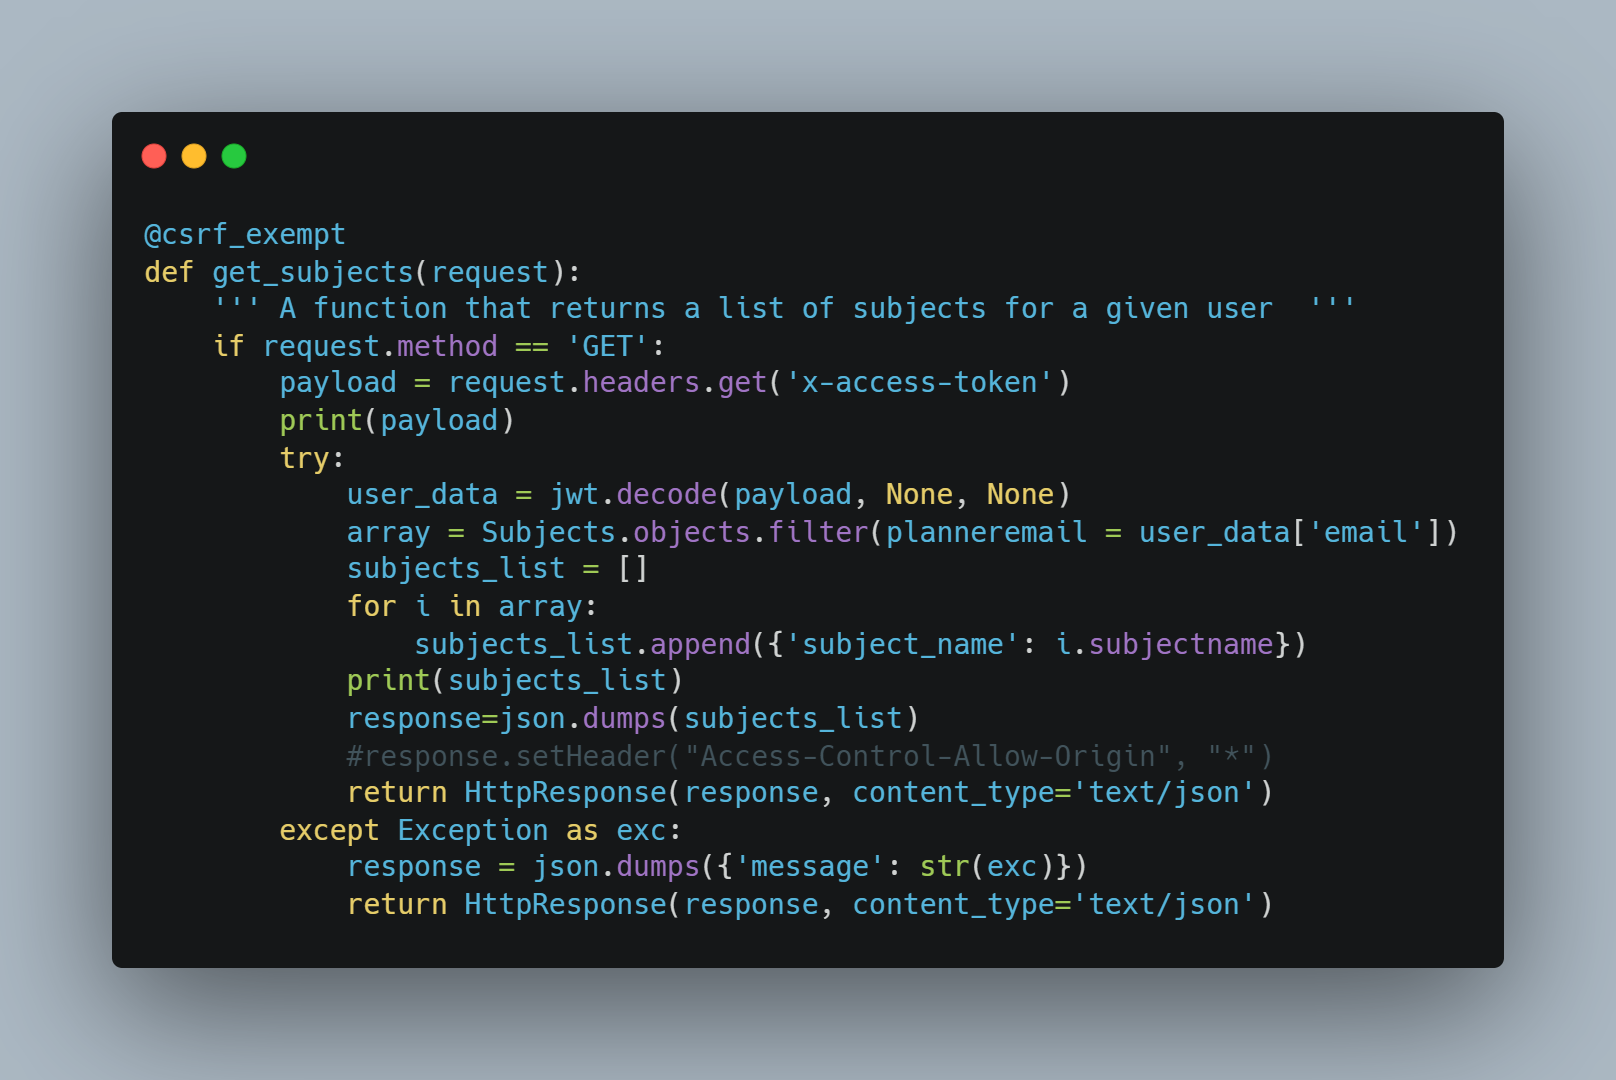
\includegraphics[width=\textwidth]{figures/BackendGet}
	\caption{Widok obsługujący zapytanie typu GET}\label{rys:BackendGet}
\end{figure}
\begin{figure}[H]
	\centering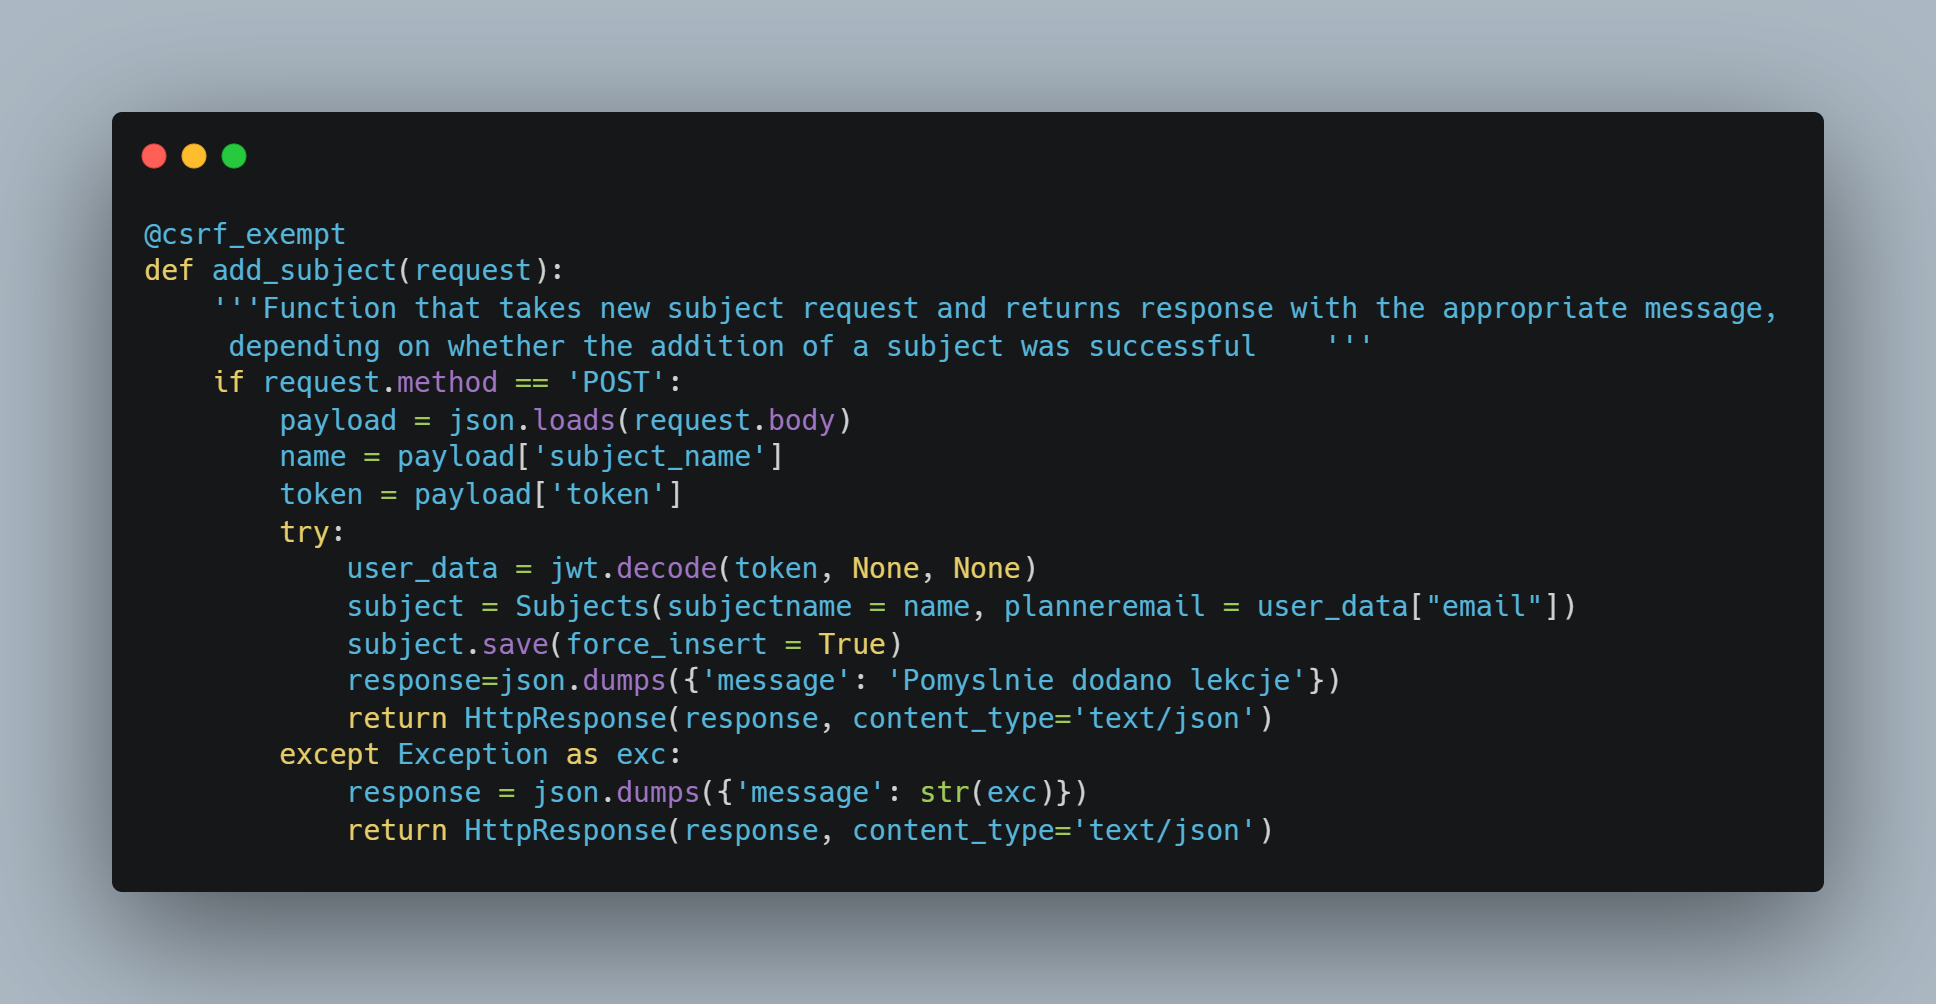
\includegraphics[width=\textwidth]{figures/BackendPost}
	\caption{Widok obsługujący zapytanie typu POST}\label{rys:BackendPost}
\end{figure}

\section{Główne funkcjonalności}
\subsection{Rejestracja i logowanie}
Rejestracja oraz logowanie zrealizowane są za pomocą dwóch adresów, co za tym idzie również dwóch widoków, obsługujących zapytania z metodą POST. Do zarejestrowania nowego użytkownika wymagane jest podanie danych takich informacji jak adres e-mail, login oraz hasło. Funkcja obsługująca rejestrację zapisuje te dane do odpowiedniej tabeli, pod warunkiem że dany użytkownik nie istnieje już w bazie danych, a nastęnie zwraca odpowiedni komunikat. W przypadku logowania wymagane jest podanie adresu e-mail oraz hasła podanych przy rejestracji. Jeśli podane dane są poprawne, generowany oraz zwracany klientowi jest token(JWT). Zakodowane w nim są wszystkie dane podane przy rejestracji, co pozwala na identyfikacje użytkownika przy dalszej komunikacji. Generacja JWT na rysunku ~\ref{rys:jwt} 
\begin{figure}[H]
	\centering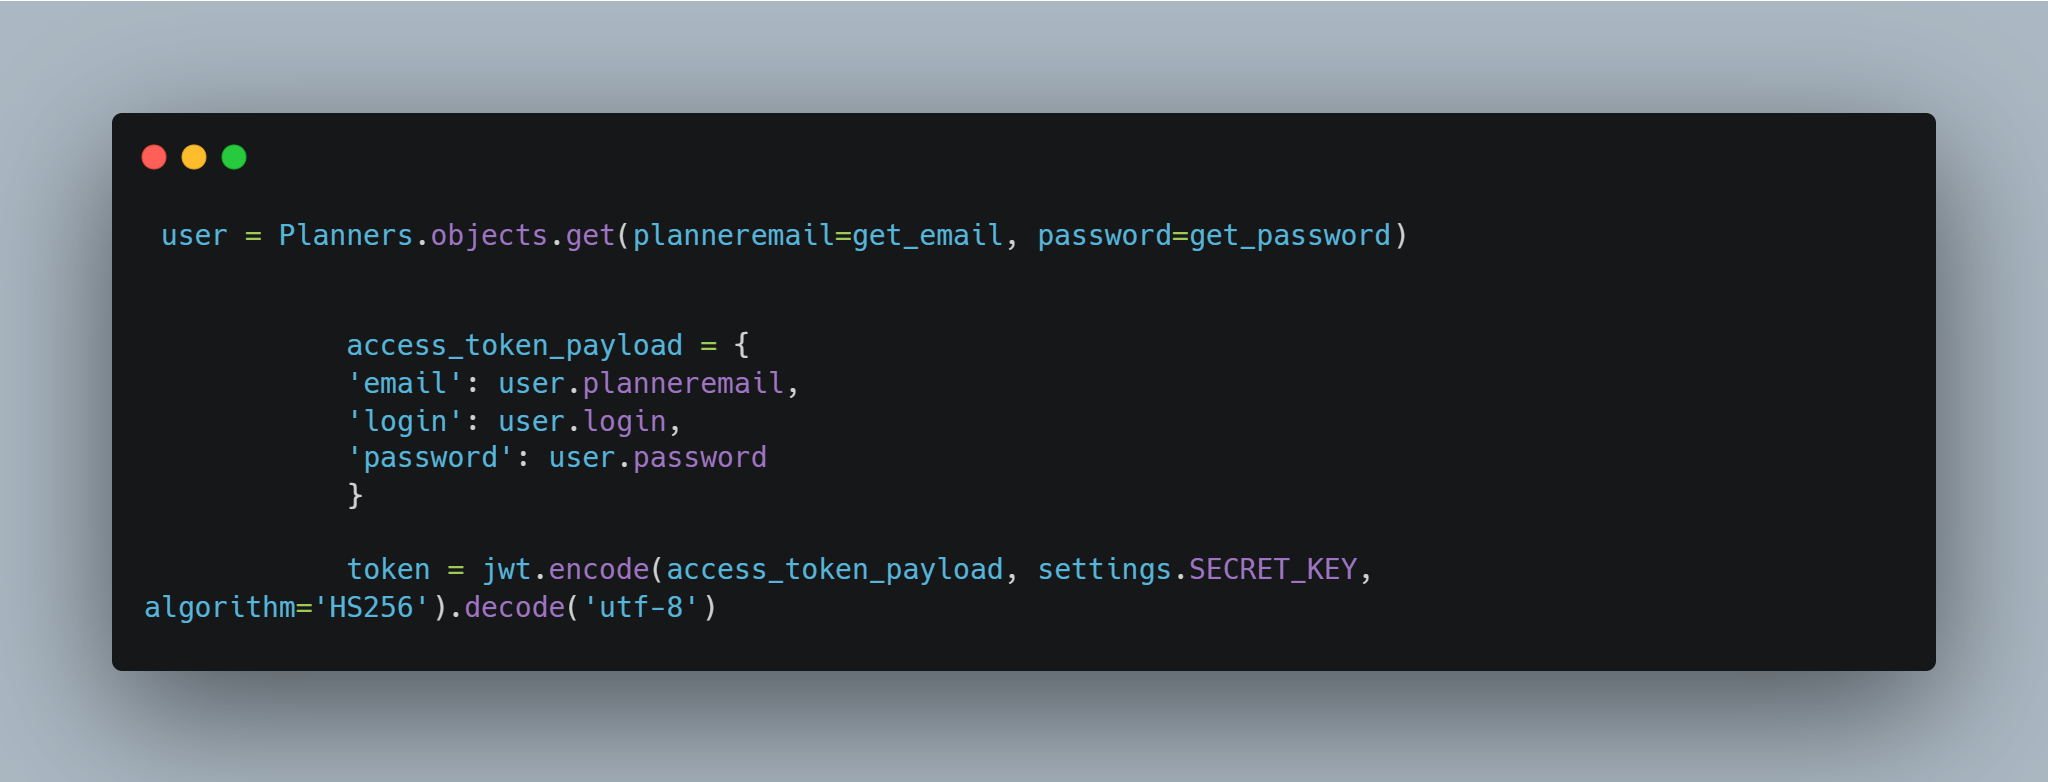
\includegraphics[width=\textwidth]{figures/jwt}
	\caption{Fragment kodu generujący JWT}\label{rys:jwt}
\end{figure}
\subsection{Uzupełnianie danych potrzebnych do generacji planu}
Dane które są wymagane do generacji planu lekcji, można podzielić na 4 grupy:
\begin{itemize}
	\item Nauczyciele
	\item Klasy
	\item Sale lekcyjne
	\item Przedmioty
\end{itemize}
w projekcie zaimplementowane są widoki, pozwalające dodawać, edytować, usuwać oraz zwracać informacje o każdej z tych grup. W większości przypadków są to proste operacje zapisu i odczytu z bazy danych, jednak w przypadku dodawania informacji o nauczycielach istnieje dodatkowa funkcjonalność, pozwalająca na wysłanie do nich wiadomości e-mail z adresem do indywidualnej ankiety, w której można określić preferowane godziny pracy. Przy pomyślnej realizacji zapytania o wysłanie wiadomości e-mail, w bazie danych tworzone są wiersze, do których zapisane będą dane z ankiet. Są one identyfikowane po unikatowym numerze, przekazywanym jako parametr w adresie URL. Dzięki takiemu rozwiązaniu, generowany jest indywidualny link do ankiety dla każdego nauczyciela.
\subsection{Generacja oraz zwracanie planów}
Generacja oraz zwracanie planów zrealizowane są za pomocą czterech widoków. Funkcja generacji planu, ma za zadanie odczytać wszystkie potrzebne informacje, i w odpowiednim formacie przekazać je do generatora. Ze względu na to że klient nie powinien oczekiwać na odpowiedź oraz że czas generacji planu może być stosunkowo długi, widok ten w przypadku pomyślnego przygotowania danych wejściowych, zwraca informację o rozpoczęciu generacji planu, nie czekając na zakończenie procesu. Dzięki temu, proces generacji nie zaburza połączenia klient-serwer. Kiedy generator skończy prace, plany lekcji zapisywane są w bazie danych w trzech wersjach, z perspektywy: klas, nauczycieli oraz sal lekcyjnych.
Każdy z tych planów, jest zwracany za pomocą pozostałych trzech widoków.

\section{Baza danych MySQL}

\chapter{Projekt i implementacja algorytmu generującego plan lekcji}

\section{Wstęp}
Problem ułożenia najlepszego planu zajęć jest problemem Np-Zupełnym. W projekcie zostało zaimplementowane podejście ewolucyjne. Na rysunek ~rysunku~\ref{rys:time_table_dia} została zobrazowana struktura generowanego planu zajęć.

\begin{figure}[h]
\centering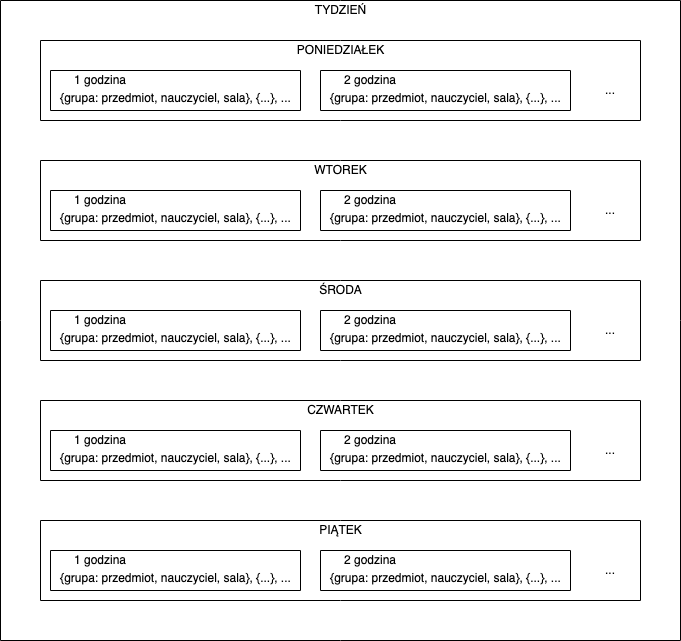
\includegraphics[width=\textwidth]{figures/time_table_dia}
\caption{Struktura planu zajęć}\label{rys:time_table_dia}
\end{figure}


Zagadnienie implementacji algorytmu można podzielić na cztery główne części: 
\begin{itemize}
	\item przygotowanie danych wejściowych,
	\item ułożenie planu zajęć,
	\item ocena planu zajęć,
	\item ewolucja planu zajęć.
\end{itemize}


\section{Przygotowanie danych wejściowych}
    
    Przygotowanie danych wejściowych jest kluczowe w działaniu algorytmu. Na podstawie danych otrzymanych od back-end, zostaje ułożona lista czteroelementowych krotek, gdzie pierwszym elementem jest nazwa grupy, drugim elementem jest nazwa przedmiotu, trzecim elementem jest nazwa nauczyciela, a czwartym elementem jest nazwa sali. Wartość elementu sali jest na początku wartością pustą null, a wartość elementu nauczyciela, jest wartością pustą null, wtedy i tylko wtedy kiedy nie został wskazany nauczyciel dla konkretnej klasy. W takiej liście znajdują się wszystkie jednostki lekcyjne występujące w całej szkole. Przykładowo jeżeli pewna klasa IIC ma mieć 5 matematyk w tygodniu z nauczycielem Jan Kowalski, to do listy dostanie dodane pięć krotek postaci (IIC, matematyka, Jan Kowalski, null). Struktura wspomnianej listy znajduje się na ~rysunku~\ref{rys:krotki}.


\begin{figure}[]
\begin{tabular}{llll}
NAZWA GRUPY & NAZWA PRZEDMIOTU & NAZWA NAUCZYCIELA & NAZWA SALI \\
IIC         & matematyka       & Jan Kowalski      & null       \\
IIC         & matematyka       & Jan Kowalski      & null       \\
IIC         & matematyka       & Jan Kowalski      & null       \\
IIC         & język polski     & Andrzej Nowak     & null       \\
IIC         & język polski     & Andrzej Nowak     & null       \\
IA          & język polski     & null              & null      
\end{tabular}
\caption{Struktura listy krotek} \label{rys:krotki}
\end{figure}

\section{Ułożenie poprawnych planów zajęć}

    Głównym założeniem układania planu zajęć jest to, że na podstawie tej samej listy krotek, zawsze zostanie wygenerowany konkretny plan zajęć. 
Układanie planu zajęć przebiega następująco:
\begin{enumerate}
	\item z listy krotek zostaje zabrana pierwsza z brzegu krotka,
	\item wybrana krotka zostaje przydzielona do pierwszej możliwej konkretnej godziny w 		\item konkretnym dniu (czyli do takiej jednostki godzinowej, wtórej są spełnione 			\item wprowadzone przez użytkownika założenia oraz jest wolna sala),
	\item poprzednie czynności zostają powtarzane tak długo, aż cała lista zostanie przeiterowana.
\end{enumerate}
Jeżeli po zakończeniu działania procesu układania planu zajęć lista krotek nie będzie pusta, to ułożony plan zajęć jest niekompletny i niepoprawny. Proces układania planu zajęć został przedstawiony na ~rysunku~\ref{rys:time_table_prep}.

\begin{figure}[h]
\centering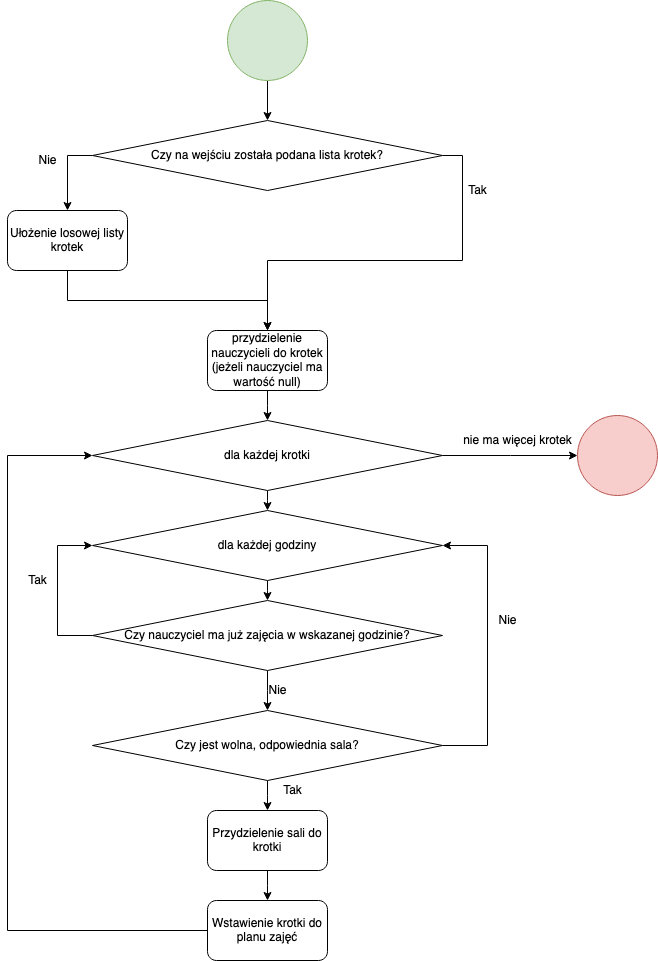
\includegraphics[width=\textwidth]{figures/time_table_prep}
\caption{Proces układania planu zajęć}\label{rys:time_table_prep}
\end{figure}

\section{Funkcja oceny}

    Funkcja oceny przyznaje planu zajęć pewną ilość punktów. Ocena może mieć wartość z zakresu od minus nieskończoności do 0, gdzie im wartość większa, tym lepsza ocena.
    Wpływ na końcową ocenę mają następujące elementy:
\begin{enumerate}
	\item liczba tzw. okienek występujących w planie zajęć każdego nauczyciela,
	\item liczba tzw. okienek występujących w planie zajęć każdej grupy,
	\item liczba trudnych przedmiotów w ciągu jednego dnia w planie zajęć każdej grupy,
	\item liczba sytuacji, w których grupa ma rozdzielone zajęcia tego samego przedmiotu innym przedmiotem (np. 1 godzina lekcyjna - matematyka, 2 godzina lekcyjna - biologia, 3 godzina lekcyjna - matematyka),
	\item liczba sytuacji, w których zajęcia wychowania fizycznego nie występują na początku lub na końcu planu zajęć dnia.
\end{enumerate}


\section{Ewolucja planów zajęć}

    Część ewolucyjna algorytmu wykorzystuje wszystkie poprzednie części. Na początku algorytm generuje pewną populację planów zajęć, która będzie nazywana dalej pierwszą generacją. Zawartość listy krotek jest identyczna dla każdej jednostki z populacji, ale kolejność krotek w liście jest pseudo losowo zmieniona. Dzięki takiemu rozwiązaniu, każda jednostka w populacji może wygenerować zupełnie inny plan zajęć. Za pomocą funkcji oceny, do każdego z planów zostaje przydzielona pewna ilość punktów. 

Połowa najgorzej ocenionych planów zostaje zabita. Z każdego planu zajęć, któremu udało się przeżyć, generowany jest kolejny plan. Plan, z którego został wygenerowany nowy plan, będzie nazywany w dalszej części pracy rodzicem, natomiast nowo wygenerowany plan będzie nazywany potomkiem. Lista krotek potomka, będzie zawierała tą samą kolejność co rodzic, ale losowo wybrane rekordy zamienią się w sposób pseudolosowy pozycjami w liście, taka zamiana będzie nazywana dalej mutacją. Nowo wygenerowane jednostki zostają ocenione oraz dodane do populacji, w ten sposób powstaje druga generacja planów zajęć.

    Czynność z poprzedniego akapitu powtarza się jeszcze g-razy, gdzie g to liczba wszystkich generacji. Działanie całego algorytmu zostało przedstawione na ~rysunku~\ref{rys:alf_flow}.


\begin{figure}[h]
\centering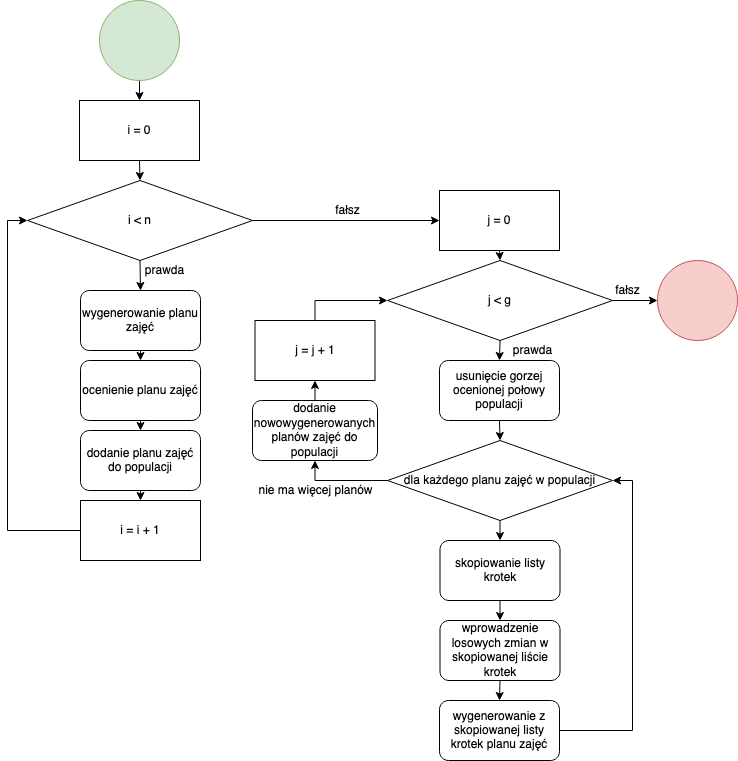
\includegraphics[width=\textwidth]{figures/alg_flow}
\caption{Algorytm - diagram}\label{rys:alf_flow}
\end{figure}





\chapter{Testowanie}
\section{Frontend}
\section{Backend}
\section{Algorytm}



\chapter{Wnioski}

Rozdziały dokumentujące pracę własną studenta: opisujące ideę, sposób lub metodę 
rozwiązania postawionego problemu oraz rozdziały opisujące techniczną stronę rozwiązania 
--- dokumentacja techniczna, przeprowadzone testy, badania i uzyskane wyniki. 

Praca musi zawierać elementy pracy własnej autora adekwatne do jego wiedzy praktycznej uzyskanej w
okresie studiów. Za pracę własną autora można uznać np.: stworzenie aplikacji informatycznej lub jej
fragmentu, zaproponowanie algorytmu rozwiązania problemu szczegółowego, przedstawienie projektu 
np.~systemu informatycznego lub sieci komputerowej, analizę i ocenę nowych technologii lub rozwiązań
informatycznych wykorzystywanych w przedsiębiorstwach, itp. 

Autor powinien zadbać o właściwą dokumentację pracy własnej obejmującą specyfikację założeń i 
sposób realizacji poszczególnych zadań
wraz z ich oceną i opisem napotkanych problemów. W przypadku prac o charakterze 
projektowo-implementacyjnym, ta część pracy jest zastępowana dokumentacją techniczną i użytkową systemu. 

W pracy \textbf{nie należy zamieszczać całego kodu źródłowego} opracowanych programów. Kod źródłowy napisanych
programów, wszelkie oprogramowanie wytworzone i wykorzystane w pracy, wyniki przeprowadzonych
eksperymentów powinny być umieszczone np. na płycie CD, stanowiącej dodatek do pracy.

\section*{Styl tekstu}

Należy\footnote{Uwagi o stylu pochodzą częściowo ze stron prof. Macieja Drozdowskiego~\cite{Drozdowski2006}.} 
stosować formę bezosobową, tj.~\emph{w pracy rozważono ......, 
w ramach pracy zaprojektowano ....}, a nie: \emph{w pracy rozważyłem, w ramach pracy zaprojektowałem}. 
Odwołania do wcześniejszych fragmentów tekstu powinny mieć następującą postać: ,,Jak wspomniano wcześniej, ....'', 
,,Jak wykazano powyżej ....''. Należy unikać długich zdań. 

Niedopuszczalne są zwroty używane w języku potocznym. W pracy należy używać terminologii informatycznej, która ma 
sprecyzowaną treść i znaczenie. 

Niedopuszczalne jest pisanie pracy metodą \emph{cut\&paste}, bo jest to plagiat i dowód intelektualnej indolencji autora.
Dane zagadnienie należy opisać własnymi słowami. Zawsze trzeba powołać się na zewnętrzne źródła. 



\chapter{Zakończenie}

Zakończenie pracy zwane również Uwagami końcowymi lub Podsumowaniem powinno zawierać ustosunkowanie
się autora do zadań wskazanych we wstępie do pracy, a w szczególności do celu i zakresu pracy oraz
porównanie ich z faktycznymi wynikami pracy. Podejście takie umożliwia jasne określenie stopnia
realizacji założonych celów oraz zwrócenie uwagi na wyniki osiągnięte przez autora w ramach jego
samodzielnej pracy.

Integralną częścią pracy są również dodatki, aneksy i załączniki zawierające stworzone w ramach pracy programy, aplikacje i projekty.


%--------------------------------------
% Literatura
%--------------------------------------

\bibliographystyle{plain}{\raggedright\sloppy\small\bibliography{bibliografia}}

%--------------------------------------
% Dodatki
%--------------------------------------

\cleardoublepage\appendix%
\newpage

\chapter{Załącznik do pracy}


%--------------------------------------
% Informacja o prawach autorskich
%--------------------------------------

\ppcolophon

\end{document}
